
\chapter{Projekt systemu}
\thispagestyle{chapterBeginStyle}

W tym rozdziale został przedstawiony dokładny projekt systemu, jest on podzielony na kilka podrozdziałów. \textbf{Grupy użytkowników} oraz \textbf{Przypadki użycia} opisują szczegółowo, do czego i przez kogo będzie mogła zostać uzyta implementowana platforma. Sekcje \textbf{Diagramy aktywności} i \textbf{Diagramy sekwencji} pokazują, w jaki sposób udało się osiągnąć bardziej skomplikowane cele określone za pomocą przypadków użycia, niektóre funkcjonalności w zależności od ich charakterystyki zostaną przedstawione na diagramach aktywności - te dotyczące programisty ze względu na bardziej skomplikowane algorytmy, natomiast na diagramach sekwecji - te nastawione na funkcjonalności biznesowe.

W kolejnych sekcjach znajdą się \textbf{Diagramy klas} oraz \textbf{Projekt bazy danych}. W pierwszej opisane zostaną klasy, które musiały zostać stworzne do implementacji procesów zdefiniowanych w wcześniejszych podrozdziałach, odpowiednio w drugiej znajdą się schematy bazy danych podzielone ze względu na funkcjonalności.

Do implementacji frameworku oraz funkcjonalności wbudowanych użyto wzorca architektonicznego \textit{model-view-controller}. Polega on na następującym podziale aplikacji: \textbf{model}, odpowiedzialny za reprezentacje problemu i logikę, \textbf{view} (widok) opisujący interfejs użytkownika oraz \textbf{controller}, który przyjmuje polecenia użytkownika i odpowiada na jego żądania za pomocą modelu i widoku. Składa się on z trzech wzorców projektowych:
\begin{itemize}
	\item kompozyt -- sposób tworzenia widoków, możliwość zagnieżdżania ich w sobie
	\item obserwator -- model może zmienić stan, o czym musi zostać powiadomiony widok (aktualizacja informacji)
	\item strategia -- wybranie strategii obsługi zapytania w kontrolerze na podstawie samego żądania
\end{itemize}
W projekcie użyto również wzorzec projektowy \textit{inversion of control (odwórcenie sterowania)}. Tworzenie egzemplarzy większości encji i serwisów obsługuje Spring Framework, o który oparty jest projekt. Wspomniane \textit{IoC} zostało zrealizowane poprzez wstrzykiwanie zależności. 

\section{Grupy użytkowników}
We frameworku możemy zdefiniować 3 grupy użytkowników, którzy będą korzystać z jego udogodnień. \textbf{Programista} jest to użytkownik frameworka, który implementuje swój sklep z pomocą narzędzi dostarczonych przez opisywany system. \textbf{Administrator} to ktoś, zajmujący się backofficową\footnote{backoffice - w systemach e-commerce panel do obsługi i utrzymania sklepu} obsługą sklepu - obsługa zamówień. \textbf{Klient} jest to końcowy aktor, który przegląda katalog i dokonuje zakupów. 

Warto zaznaczyć w tym momencie, że tematem pracy jest zaimplementowanie frameworka, co wskazuje na to, że funkcjonalności będą skupione głównie na programiście i administratorze. Przypadki użycia powiązane z klientem są zmienną w implementowanym systemie. Oznacza to nic innego, że rola klienta jest uzależniona od konfiguracji i dodatków systemu. Głównym celem jest to, aby stworzyć narzędzie dzięki, któremu możliwości administratora systemu i klienta są ograniczone jedynie \textit{fantazją} programisty. Założenie to bardzo dobrze ilustruje następujący przykład:
\begin{example}
	Załóżmy, że implementujemy sklep internetowy, korzystając z opisywanego frameworka. Nasz pracodawca życzy sobie aby w sklepie pojawił się również blog z artykułami, którymi będzie można zarządzać w panelu administracyjnym. Normalnie proces implementacji takiej funkcjonalności wiązałby się z przygotowaniem modelu w bazie danych i pełnej jego obsługi, również ze strony front-endowej. Z użyciem frameworka proces można skrócić do zaimplementowania modelu i paru prostych komend aby wygenerować mechanizm do manipulacji stworzonym modelem, czyli możliwość dodania, usunięcia i edycji dowolnego blogu w panelu administracyjnym.
\end{example}

\section{Przypadki użycia}
Jak zostało zdefiniowane w poprzednim punkcie, w pracy przewidziano 3 grupy użytkowników. W zamyśle framework jest narzędziem dla programisty, jednak w systemie został zaimplementowany szereg rozwiązań gotowych do wykorzystania dla końcowych użytkowników, dlatego diagramy przypadków użycia zostały podzielone na trzy klasy: 
\begin{itemize}
	\item przypadki użycia Programisty 
	\item przypadki użycia Użytkownika Administracyjnego potencjalnego serwisu e-commerce, opartego na opisywanym Frameworku
	\item przypadki użycia użytkownika końcowego, czyli Klienta
\end{itemize}
Na rysunku \ref{useCaseProgrammer} zostały przedstawione najważniejsze przypadki użycia frameworku. Programista ma swobodny dostęp do rozszerzania encji, w szczególności klasy Produkt, która ma wyjatkowo strategiczne znaczenie w systemach e-commerce. Dodatkowo ma możliwość uczynienia niestandardowych pól wyszukiwalnymi przez klienta. Sytuacja została zobrazowana na poniższym przykładzie.
\begin{example}
	Załóżmy, że mamy niestandardowe pole proste (String) w encji klasyfikowanej przez twórców ewentualnego sklepu związanego z opisywanym frameworkiem jako finalna encja nadająca się do sprzedaży. Niech ta encja nazywa się \texttt{MyProduct extends Product} z polem \texttt{myCustomField}. Jedyne co w tej sytuacji musimy zrobić, aby system mógł wyciągnąć wartość tego pola i uczynić je wyszukiwalnym, to wpisać do tabeli zawierającej indeksowane cechy produktu nazwę danego pola, system za pomocą refleksji\footnote{\textit{refleksja} ( eng. reflection) -- udogodnienie w języku Java, pozwalające na wyświetlenie i manipulacje właściwościami klasy. Więcej w sekcji \textbf{słowniczek}.} wyekstrahuje wartość pola z encji i umożliwi wyszukanie produktu na sklepie
\end{example}

Dodane przez Programistę encje są obsługiwane przez framework, dodatkowo po dodaniu specjalnej adnotacji\footnote{adnotacja -- używane w języku Java od wersji 1.7, najczęściej służą do określania dodatkowych właściwości pól bądź klas} nad deklaracją jej klasy w kodzie, może być zarządzana w uniwersalnym panelu administracyjnym. Osoba zajmująca się implementacją sklepu opartego o opisywaną platformę może również uruchomić dowolną \textit{(skończoną)} ilość instancji Apache Solr, czyli bazy danych noSQL, służącej do obsługiwania zapytań związanych z katalogiem produktowym (skalowalność pionowa tylko tej części aplikacji, która tego potrzebuje). W odniesieniu do przypadku użycia \textit{Nadpisanie mechanizmu wyszukiwania} z rysunku \ref{useCaseProgrammer} serwisy są oparte na interfejsach, zapewniając Programiście możliwość nadpisania jego logiki zgodnie z zasadami polimorfizmu. 

\begin{figure}
\begin{center}
	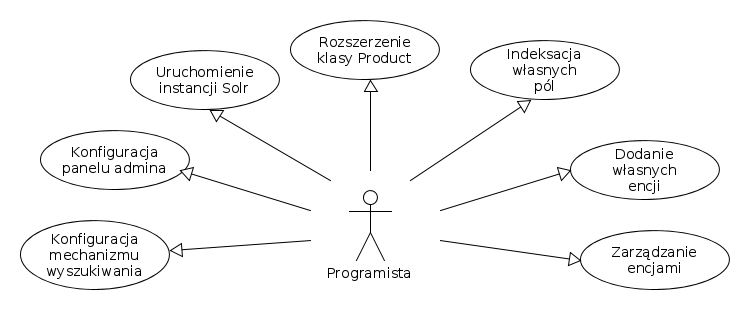
\includegraphics[width=1\textwidth]{ucdev.png}
\end{center}
\caption{{\color{black}Diagram przypadków użycia związany z Programistą.}} \label{useCaseProgrammer}
\end{figure}
\begin{figure}
	\begin{center}
		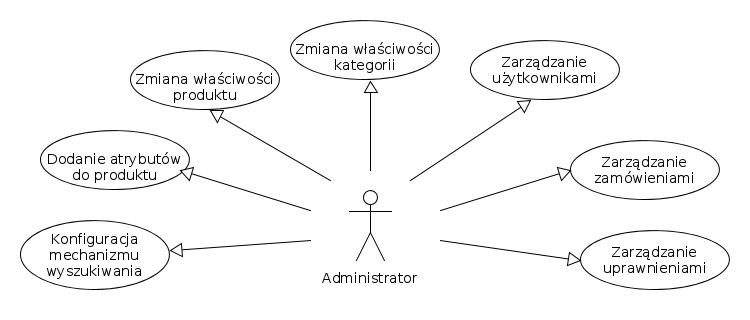
\includegraphics[width=1\textwidth]{ucadmin.png}
	\end{center}
	\caption{{\color{black}Diagram przypadków użycia związany z Administratorem ewentualniego systemu.}} \label{useCaseAdmin}
\end{figure}
Rysunek \ref{useCaseAdmin} przedstawia przypadki użycia z punktu widzenia Administratora potencjalnego systemu. Z punktu widzenia platformy jest to również klient, gdyż framework zakłada, że nie ma on wiedzy technicznej i nie potrafi programować. Podobnie jak programista, może konfigurować mechanizm wyszukiwania, jednak bardziej wysokopoziomowo, np. deklaracja używanych facetów. Panel administracyjny zakłada zarządanie najważniejszymi encjami: produkt, kategoria, użytkownik, zamówienie, uprawnienie i parę innych.

Diagram na rysunku \ref{useCaseCustomer} dotyczy przypadków użycia elementów frameworku przez końcowego użytkownika. Są to klasyczne funkcjonalności tradycyjnego sklepu internetowego. \textit{Wyszukanie produktu} zostało zaprojektowane, tak aby możliwy był również do zaimplementowania mechanizm podpowiedzi i podświetlania. Apache Solr udostępnia taką funkcjonalność. \textit{Złożenie zamówienia} dotyczy opisanego w rozdziale \textbf{Analiza problemu} kłopotu z archwizacją produktu, został on rozwiązany prostym mechanizmem wersjonowania. 
\begin{figure}
	\begin{center}
		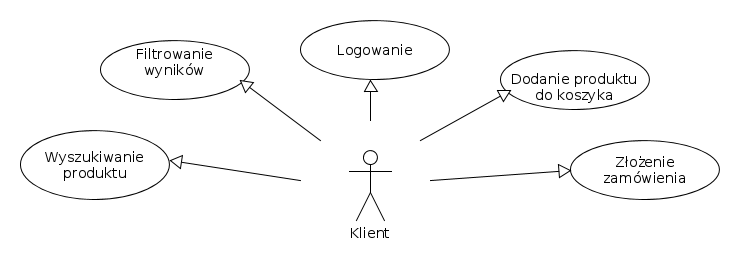
\includegraphics[width=1\textwidth]{uccustomer.png}
	\end{center}
	\caption{{\color{black}Diagram przypadków użycia związany z Klientem końcowym ewentualniego systemu.}} \label{useCaseCustomer}
\end{figure}

Diagramy typu \textit{use-case} ściśle wiążą się z wymaganiami funkcjonalnymi systemu. Jest wiadome, że można je również sklasyfikować pod względem aktorów występujących w systemie, dlatego też powiązania przypadków użycia z wymaganiami funkcjonalnymi zostały umieszczone na diagramie z rysunku \ref{wymtoUC}. Na diagram należy patrzeć poziomo, po zapoznaniu się z legendą. Wymagania są w nieprzypadkowej kolejności, są ustawione od lewej do prawej. Im bardziej na prawo, tym wymaganie jest bardziej biznesowe, im bardziej na lewo -- dotyczą rdzeniowych elementów platformy. Warto zauważyć zależność, że im dalej patrzymy na diagram, tym więcej niebieskich i żółtych \textit{use case'ów} -- tych zarezerwowanych dla Administracji i Klientów rozwiązania e-commerce. Natomiast im bardziej na lewo tym więcej czerwonego, czyli przypadków przemyślanych dla Programisty.
\begin{figure}
	\begin{center}
		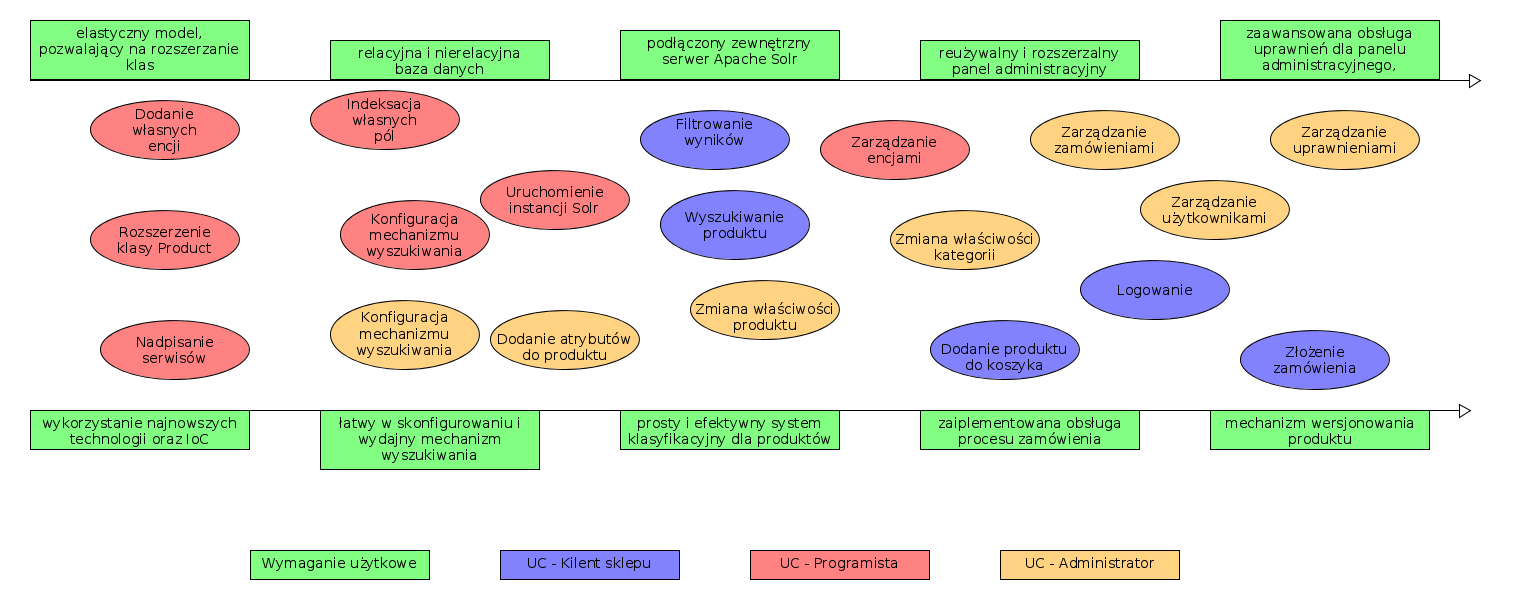
\includegraphics[angle=270,scale=0.4]{wymToUC.png}
	\end{center}
	\caption{{\color{black}Diagram przypadków użycia związany z wymaganiami funkcjonalnymi}} \label{wymtoUC}
\end{figure}

Jak zostało wspomniane wcześniej w sekcji \textbf{Grupy użytkowników i założenia}, framework jest narzędziem głównie dla programisty, to on zdecyduje co ma się znajdować w finalnym systemie, dlatego w niniejszym podrozdziale zostaną rozwinięte przypadki użycia dla programisty związane z obsługą i oprogramowywaniem dynamicznych elementów platformy. Jest to odpowiedź na najtrudniejsze z wymagań, czyli \textbf{elastyczny model, pozwalający na rozszerzenie klas} oraz \textbf{reużywalny i rozszerzalny panel administracyjny}.
\subsection{Dynamiczna tabela encyjna}
Dynamiczna tabela encyjna jest autorskim rozwiązaniem, służącym do wylistowywania dowolnych encji związanych z systemem w panelu administracyjnym, wiążą się z nim przpadki użycia z rysunku \ref{dynEntTabUC}
\begin{figure}[H]
	\begin{center}
		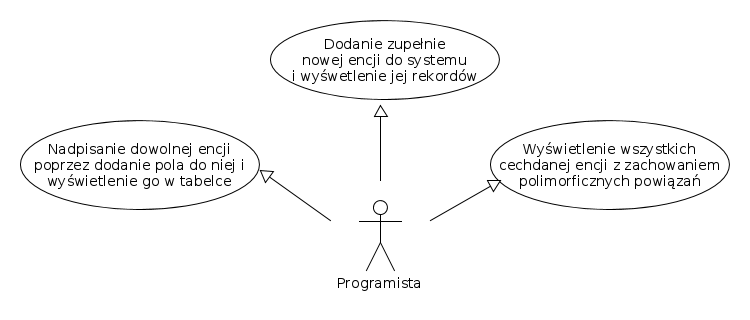
\includegraphics[scale=0.5]{dynEntTabUC.png}
	\end{center}
	\caption{{\color{black}Diagram przypadków użycia związany z dynamiczą tabelą encyjną}} \label{dynEntTabUC}
\end{figure}

\subsection{Dynamiczny formularz encyjny}
Dynamiczny formularz encyjny to kolejne autorskie rozwiązanie, służące do dodawania edycji i wyświetlania szczegółów encji związanych z systemem w panelu administracyjnym, wiążą się z nim przpadki użycia z rysunku \ref{dynEntFormUC}
\begin{figure}[H]
	\begin{center}
		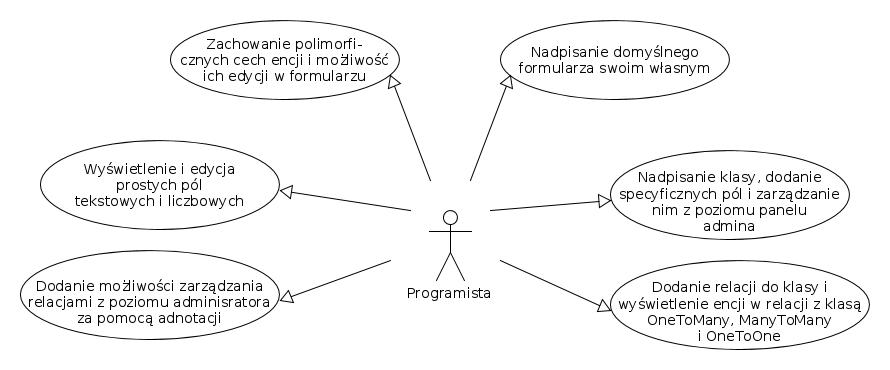
\includegraphics[scale=0.5]{dynEntFormUC.png}
	\end{center}
	\caption{{\color{black}Diagram przypadków użycia związany z dynamicznym formularzem encyjnym}} \label{dynEntFormUC}
\end{figure}

\subsection{Manipulacja produktem}
Produkt w implementowanym systemie jest to encja bardzo dynamiczna, łatwo konfigurowalna. Wiążą się z nim przypadki użycia znajdujące się na rysunku \ref{manipProd}
\begin{figure}[H]
	\begin{center}
		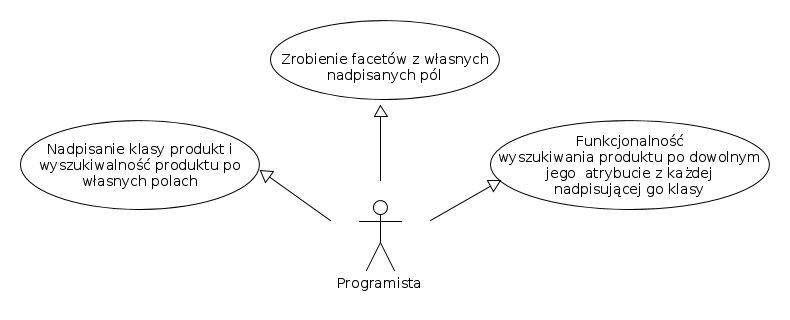
\includegraphics[scale=0.5]{manipProd.png}
	\end{center}
	\caption{{\color{black}Diagram przypadków użycia związany z dynamicznym formularzem encyjnym}} \label{manipProd}
\end{figure}

\section{Diagramy aktywności}
W tej sekcji zostały przedstawione diagramy aktywności dla najbardziej skomplikowanych logicznie elementów systemu. Dynamiczna tabela i formularz opisany w poprzednim podrozdziale wymagają skomplikowanych operacji, aby mogły pozostać ogólne i elastyczne na tyle ile być powinny. Oznacza to, że muszą obsługiwać zmiany w modelu wywołane przez osoby trzecie - \textbf{programistów}. W niniejszym podrozdziale przedstawiono działanie algorytmów stojących za dynamicznymi elementami platformy.

\subsection{Wyszukiwanie cech produktu}
Ta sekcja odnosi się do przypadków użycia związanych z podrozdziałem \textbf{Manipulacja produktem}. Wytłumaczono tutaj jak osiągnięto założoną elastyczność przy konfigurowaniu encji reprezentującej produkt w sklepie. 

Każdy Produkt w systemie jest indeksowany, oznacza to, że z relacyjnej bazy danych, wraz ze swoimi wszystkimi atrybutami trafia do nierelacyjnych dokumentów wyszukiwarki Solr na osobnym serwerze, aby odciążyć aplikacje w razie dużego ruchu. Zebranie wszystkich atrybutów produktów to skomplikowane zadanie, gdyż jego cechy mogą być ukryte w następujących miejscach: 
\begin{itemize}
	\item atrybuty dziedziczone po atrybutach klasyfikacyjnych kategorii, w której się znajduje
	\item atrybuty dziedziczone po wszystkich przodkach swojej kategorii
	\item własne pola i pola wszystkich klas, które nadpisały Produkt 
\end{itemize}  

Zadanie to wymaga zejścia do poziomu refleksji w Javie, jednak ten temat zostanie poruszony później. Wyszukiwanie wszystkich atrybutów obsługuje algorytm, którego diagram aktywności został umieszczony na rysunku \ref{diagramaktywIndeks}

Pierwszym krokiem jest znalezienie wszystkich produktów, co nie jest również oczywistym zadaniem, gdyż nie jest wiadome jaką klasę ma finalny produkt, mógł zostać nadpisany przez programistę, który w swojej klasie zdefiniował pewne pola, które również muszą zostać uwzględnione przy indeksacji produktów. Po znalezieniu \textit{klasy sufitowej} (czyli najwyższej w abstrakcji) mamy pewność, że wszystkie niestandardowe pola znajdą się w obiekcie pobranym przez nas z bazy danych. Z bazy danych muszą zostać również pobrane pola zadeklarowane jako te, które są wyszukiwalne w sklepie (oczywiste jest, że powinno się mieć wybór, które pola z produktu trafią do sklepu, a które nie). Mając te dwie rzeczy, jest możliwe wyciągnięcie z obiektu, którego klasa nie jest znana, wszystkich interesujących nas pól. Wszystkie wyciągnięte wartości następnie trafiają do dokumentu wyszukiwarki. Nie jest to jeszcze koniec, gdyż zostają wciąż do wyciągnięcia cechy produktu z systemu klasyfikacyjnego, zostało to zrealizowane algorytmem przejścia po drzewie. Wszystkie cechy produktu są dodawane do listy dokumentów (jeden dokument - jeden produkt) i są wysyłane na serwer Apache Solr. Przykład skąd mogą pochodzić cechy produktu został umieszczone na rysunku \ref{cechyProd}.
\begin{figure}
	\begin{center}
		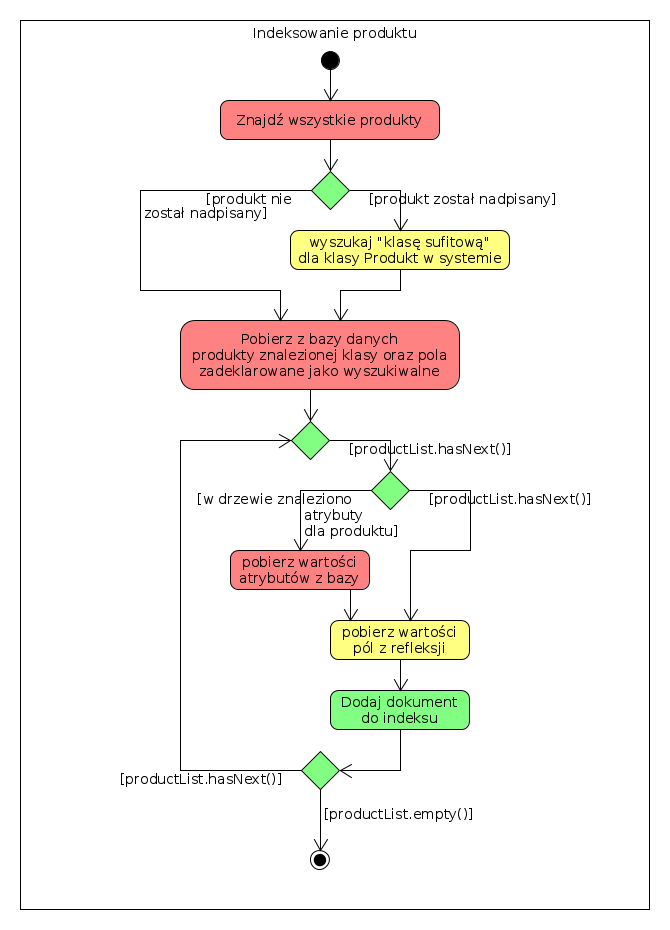
\includegraphics[scale=0.5]{diagramaktywIndeks.png}
	\end{center}
	\caption{{\color{black}Diagram aktywności opisujący algorytm znajodwania wszystkich atrybutów produktu}} \label{diagramaktywIndeks}
\end{figure}
\begin{figure}
	\begin{center}
		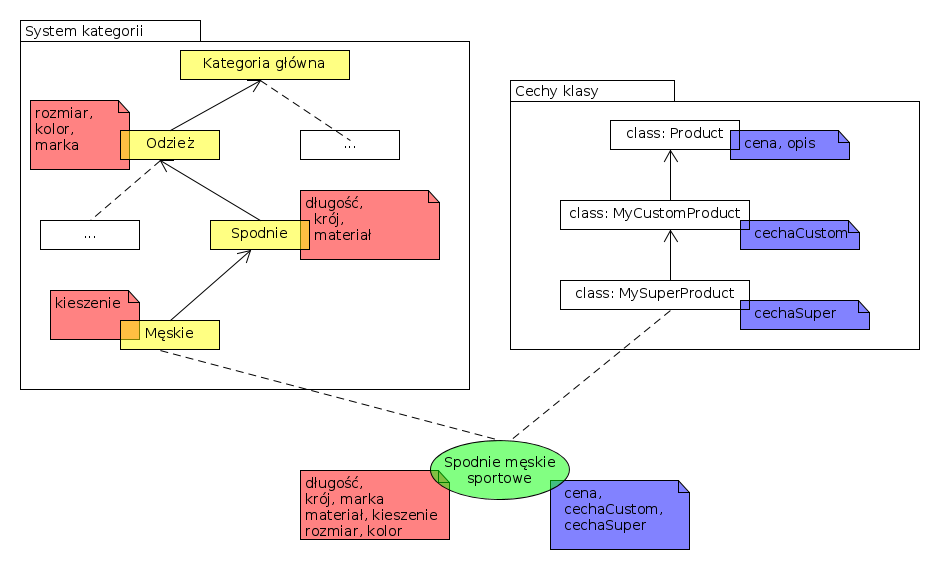
\includegraphics[scale=0.5]{cechyProd.png}
	\end{center}
	\caption{{\color{black}Diagram przykładowy skąd mogą pochodzić cechy produktu}} \label{cechyProd}
\end{figure}

\subsection{Konstrukcja zapytania dynamicznego Apache Solr}
Na diagramach use case zostały opisane możliwości konfiguracji mechanizmu wyszukującego. Zdefiniowane wymagania zrealizowano za pomocą konstrukcji dynamicznego zapytania. W prostych słowach chodzi tu o kwerendę zwracającą produkty przy wyszukiwaniu. Diagram na rysunku \ref{konsDynZapy} przedstawia algorytm tworzący te zapytania. Pierwszy etap nasuwa podejrzenie, że w bazie danych musi istnieć tabela z wylistowanymi polami, które będą wyszukiwalne w sklepie. Jest to jak najbardziej trafne przypuszczenie. Dodatkowo w tabeli zostały umieszczone dodatkowe ustawienia dla pól wyszukiwania, aby mechanizm mógł być w pełni konfigurowalny. 
\begin{figure}
	\begin{center}
		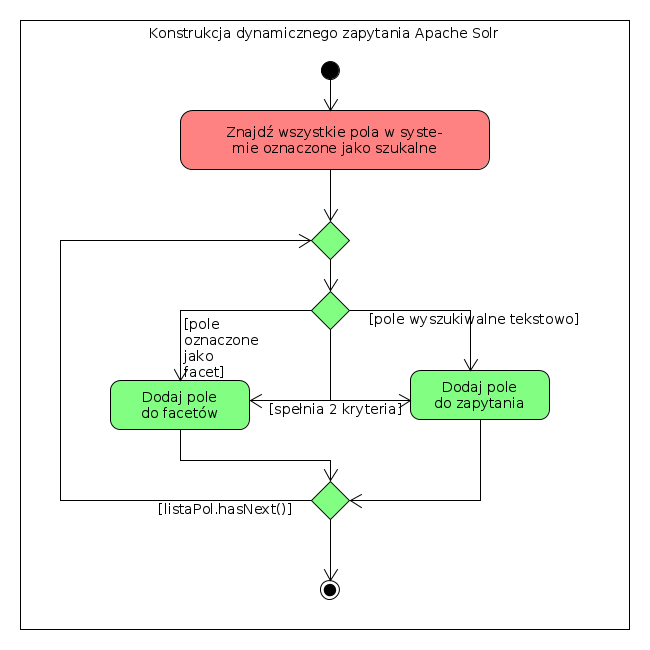
\includegraphics[scale=0.5]{konsDynZapy.png}
	\end{center}
	\caption{{\color{black}Diagram przedstawiający algorytm kostrukcji dynamicznego zapytania Apache Solr}} \label{konsDynZapy}
\end{figure}
\subsection{Konstrukcja dynamicznej tabeli encyjnej}
Dynamiczna tabela encyjna, której przypadki użycia opisano w poprzednim podrozdziale, jest wbrew pozorom zadaniem analogicznym do wyciągania cech z produktu. Ułatwieniem jest to, że w tabeli nie uwzględnia się atrybutów z systemu klasyfikacyjnego, gdyż dotyczy on tylko produktów, niestety utrudnieniem pozostaje fakt, że nie jest wiadome jakie klasy dokładnie powinny być wyświetlone w tabelach. Jedyne na czym polega system to tabela konfiguracyjna z kodami klas, które mają zostać wyświetlone w panelu administracyjnym. Proces został opisany na diagramie z rysunku \ref{konsTabEnc}. 

Najpierw szukane są encje z rodzaju podanego we wspomnianej tablei, następnie refleksją wyciąga się jej pola zaznaczone przez programistę jako te, które chce wyświetlić w tabeli jako nagłówki. Ze znalezionej listy obiektów pobiera się wartości pól, które znajdują się w nagłówkach.
\begin{figure}
	\begin{center}
		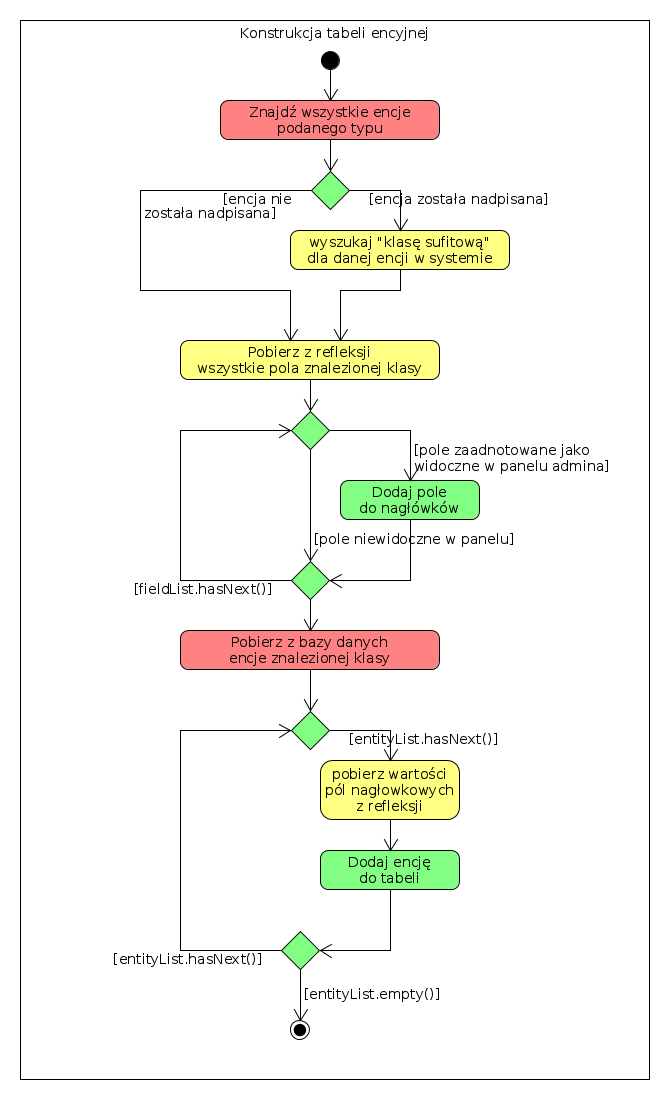
\includegraphics[scale=0.5]{konsTabEnc.png}
	\end{center}
	\caption{{\color{black}Diagram aktywności opisujący algorytm wyszukujący cechy encji uwzględnianych w tabeli.}} \label{konsTabEnc}
\end{figure}

\newpage
\subsection{Konstrukcja dynamicznego formularza encyjnego} \label{s_konDynForm}
Odbywa się to na bardzo podobnej zasadzie, jak konstrukcja tabeli. Jednak poza polami prostymi zaznaczonymi jako widzialne w panelu administracyjnym, problem stanowią relacje, które trzeba wyświetlić. Aby zachować rozszerzalność, w platformie zostały zastosowane mechanizmy z dwóch poprzednich przykładów. Po znalezieniu listy pól danej klasy, następuje tu jeszcze sklasyfikowanie ich względem tego, czy są to pola z relacjami czy nie (np. lista cen w produkcie). Wiadome jest, że relacji nie można przedstawić w postaci pola tekstowego, dlatego potrzebujemy wtedy ręcznie doczytać kolekcję w relacji z encją, której detale są wyświetlane. Wszystkie kolekcje w systemie są leniwe (ze względu na performance), dlatego przy manipulacji encją jej duże elementy takie jak listy czy zbiory są doczytywane dopiero w momencie ich użycia\footnote{ponieważ wymagają joinów, a wiadome jest że join to iloczyn kartezjański, oczywiście odpowiednio napisany nie będzie dokładnie tym samym jednak w każdym wypadku jest to duże obciążenie}. W zwykłej sytuacji framework Hibernate\footnote{Hibernate -- framework używany do komunikacji aplikacji z bazą danych} sam doczytałby tę kolekcję, jednak przy tak dużej ogólności rozwiązania nie jest to możliwe, gdyż na poziomie dynamicznego formularza nie ma on wystarczających informacji do wykonania tej operacji. Schemat algorytmu konstruującego formularz edycji encji został umieszczony na rysunku \ref{konsFormEnc}.
\newpage
\begin{figure}
	\begin{center}
		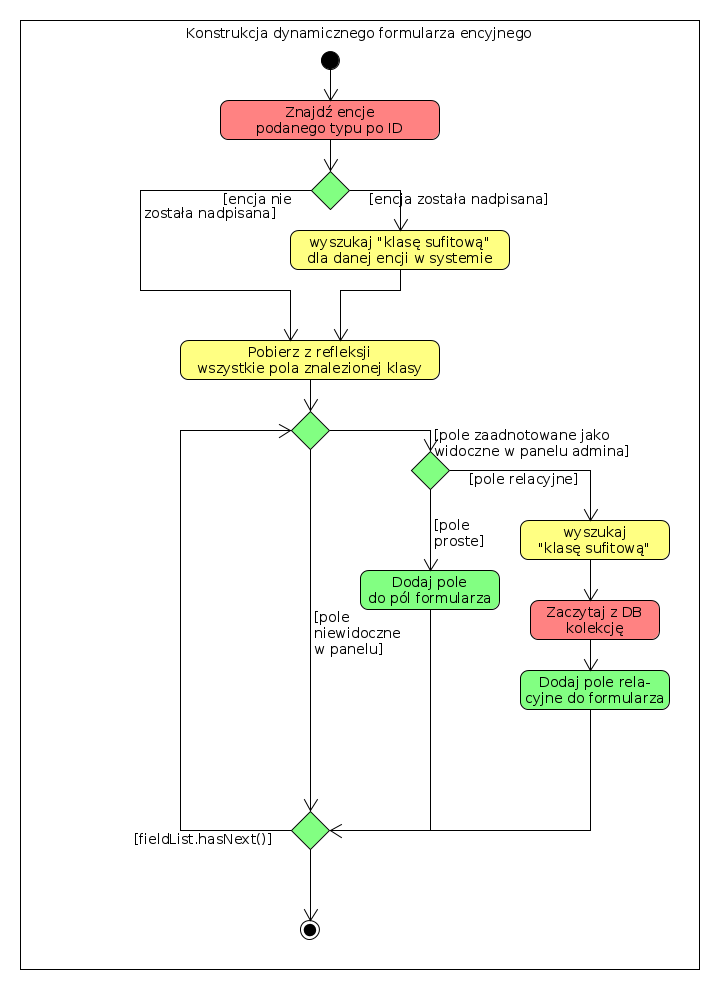
\includegraphics[scale=0.5]{konsFormEnc.png}
	\end{center}
	\caption{{\color{black}Diagram aktywności opisujący algorytm wyszukujący cechy encji uwzględnianych w tabeli.}} \label{konsFormEnc}
\end{figure}

\subsection{Podsumowanie diagramów aktywności}
Diagramy aktywności i zaprezentowane rozwiązania w nich pokrywają pewne przypadki użycia, w tej sekcji zostanie podkreślone jak przedstawione algorytmy spełniają zdefiniowane use case'y.

Patrząc na sekcję \textbf{Wyszukiwanie cech produktu} i \textbf{Konstrukcja zapytania dynamicznego Apache Solr} zostały zrealizowane następujące przypadki użycia:
\begin{itemize}
	\item Programisty: 
	\subitem Rozszerzenie klasy produkt
	\subitem Konfiguracja mechanizmu wyszukiwania
	\subitem Indeksacja własnych pól
	\item Administratora:
	\subitem Konfiguracja mechanizmu wyszukiwania
	\subitem Dodanie atrybutów do produktu
	\subitem Zmiana właściwości produktu
	\item Klienta sklepu
	\subitem Wyszukiwanie produktu
	\subitem Firtrowanie wyników
\end{itemize}

Sekcja \textbf{Konstrukcja dynamiczniej tabeli encyjnej} i \textbf{Konstrukcja dynamicznego formularza encyjnego} pokryły następujące przypadki użycia:
\begin{itemize}
	\item Programisty: 
	\subitem Konfiguracja panelu administracyjnego
	\subitem Dodanie własnych encji
	\subitem Zarządzanie encjami
	\item Administratora:
	\subitem Zmiana właściwości kategorii
	\subitem Zarządzanie użytkownikami 
	\subitem Zarządzanie zamówieniami
	\subitem Zarządzanie uprawnieniami
\end{itemize}

W podrozdziale opisującym przypadki użycia opisano również przypadki w sekcjach o dynamicznym formularzu, tabeli i manipulacji produktem, oczywiste jest, że wspomniane użycia bezpośrednio wiążą się z opisanymi komponentami.

Realizacja przypadków użycia, których nie mogły pokryć algorytmy opisane w niniejszym podrozdziale ze względu na swoje biznesowe pochodzenie, zostaną opisane na diagramach sekwencji. 
\newpage
\section{Diagramy sekwencji}

W tej sekcji zostały przedstawione diagramy sekwencji dla poszczególnych elementów systemu, mają one razem z diagramami aktywności zrealizować wszystkie przypadki użycia. Diakramy sekwencji dobrze oddają sens funkcjonalności biznesowych i właśnie ich dotyczy ta sekcja. 

\subsection{Zmiana właściwości dowolnej encji}
W każdym systemie bazodanowym, konieczna jest manipulacja encjami. We wcześniejszych rozdziałach zostało wprowadzone pojęcie dynamicznych tabel i formularzy edycyjnych. Z punktu widzenia bazy danych, nie ma dużego znaczenia jaka encja jest edytowana, zarówno Produkt jak i Kategoria to jedynie zbiór krotek w tabeli relacyjnej, dlatego właśnie zdecydowano się na generyczny mechanizm modyfikacji encji. W prostych słowach, w systemie nie ma osobnych formularzy edycyjnych dla poszczególnych encji, są one generowane na podstawie kodu Javowego. 

Funkcjonalność zmiany właściwości dowolnej encji zostanie omówiona na przykładzie zmiany nazwy produktu, ale jak już wyżej zostało wspomniane, ten sam mechanizm działa dla dowolnej encji, która może być modyfikowana przez framework. Po zalogowaniu się i wyświetleniu menu, administrator wybiera dowolny produkt, po czym zmienia dane pole w formularzu edycji i następnie zapisuje produkt. Diagram \ref{zmianaWlEncji} przedstawia cały proces. Najważniejsze etapy to 5 oraz od 8 do 13, to one odpowiedzialne są za elastyczność systemu - każda encja jest modyfikowana w ten sam sposób - generycznie, przez refleksję. W tym miejscu widać główny cel i zamysł pracy: system jest siadomy tego jaki obiekt edytuje, dlatego może mieć dostęp do jego właściwości (9. findPolimorficFieldsOf) - metoda ta zwraca wszystkie możliwe pola dla danego obiektu, właśnie dlatego, gdy programista nadpisze jakąś klasę, która jest używana w systemie, funkcjonalności modyfikacji encji zostaną zachowane, gdyż framework będzie w stanie wyciągnąć z obiektu każde nowe pole. Mechanizm ten zastosowany jest również we wszystkich kluczowych funkcjonalnościach, co skutkuje bardzo elastycznym modelem.
\begin{figure}
	\begin{center}
		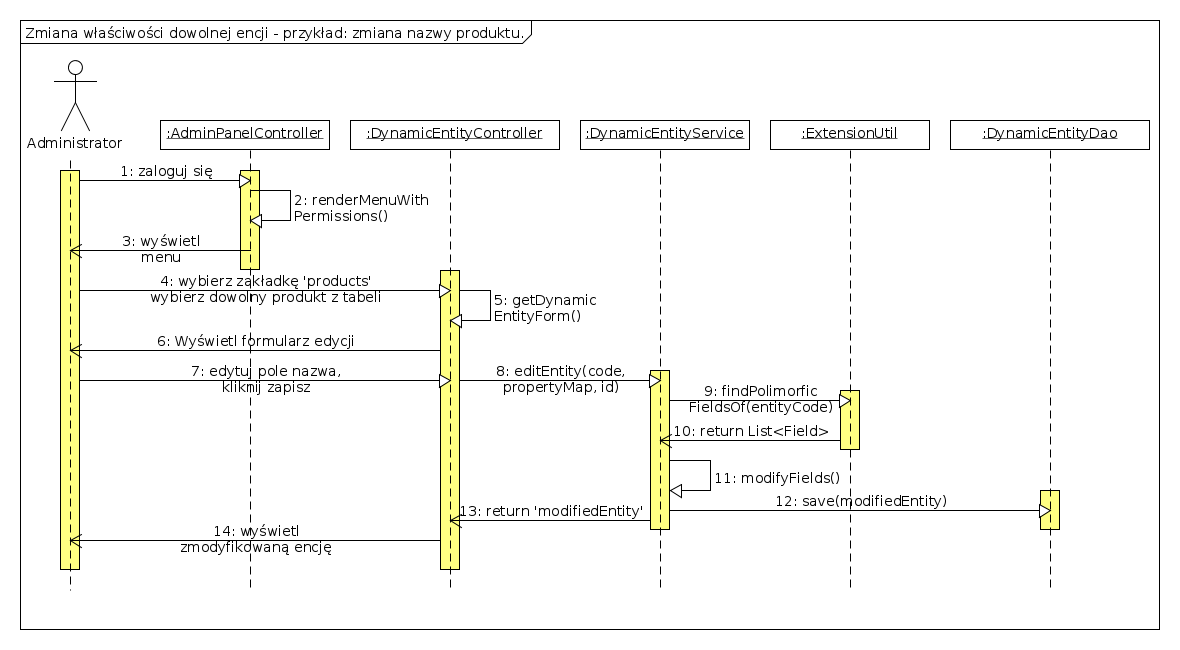
\includegraphics[scale=0.4]{zmianaWlEncji.png}
	\end{center}
	\caption{{\color{black}Diagram sekwencji opisujący opiisujący zmianę właściwości dowolnej encji na przykładzie produktu.}} \label{zmianaWlEncji}
\end{figure}

\subsection{Modyfikacja dowolnej relacji encji}
Dynamiczny formularz encyjny omówiony na diagramach aktywności zawiera również pola relacyjne, rysunek \ref{zmianaWRel} przedstawia diakram sekwencji zmiany w relacji dowolnej encji na przykładzie dodania dziecka do kategorii. Okazuje się to być dużym problemem dla frameworka, gdyż modyfikowany jest obiekt klasy kategoria (\texttt{Category}) i tylko na tej podstawie potrzeba określić jakie ma relacje i co więcej, wyciągnąć je z bazy danych. Problem został rozwiązany poprzez wprowadzenie do systemu dodatkowych parametrów adnotacji \texttt{@AdminVisible}, która jest odpowiedzialna za oznaczanie w kodzie Javowym pól klas, które zostaną wyświetlone w tabeli i formularzu edycyjnym. Za etap wyciągnięcia relacji, które pojawią się w formularzu edycji odpowiada punkt 5 na rysunku \ref{zmianaWRel}. Następnie dla wszystkich encji relacyjnych (np. produkty powiązane z kategorią) zostaje zbudowana dynamiczna tabela - tylko że wewnątrz formularza edycyjnego (pkt. 6 do 8). Następnie po kliknięciu \textit{add} przy tabelce z relacją, pobierana jest lista możliwych do przypisania encji i w przypadku kliknięcia na dany rekord, zostaje on wprowadzony w relację z edytowaną encją. Kolejne punkty odpowiadają za elastyczność rozwiązania, czyli ponownie (jak w poprzednich funkcjonalnościach), dla każdej znalezionej encji należy znaleźć klasę sufitową i to na jej tworzyć powiązania. Formularz edycyjny jest przedstawiony w formie pól tekstowych, checkboxów i tabelek z relacjami.
 \begin{figure}
 	\begin{center}
 		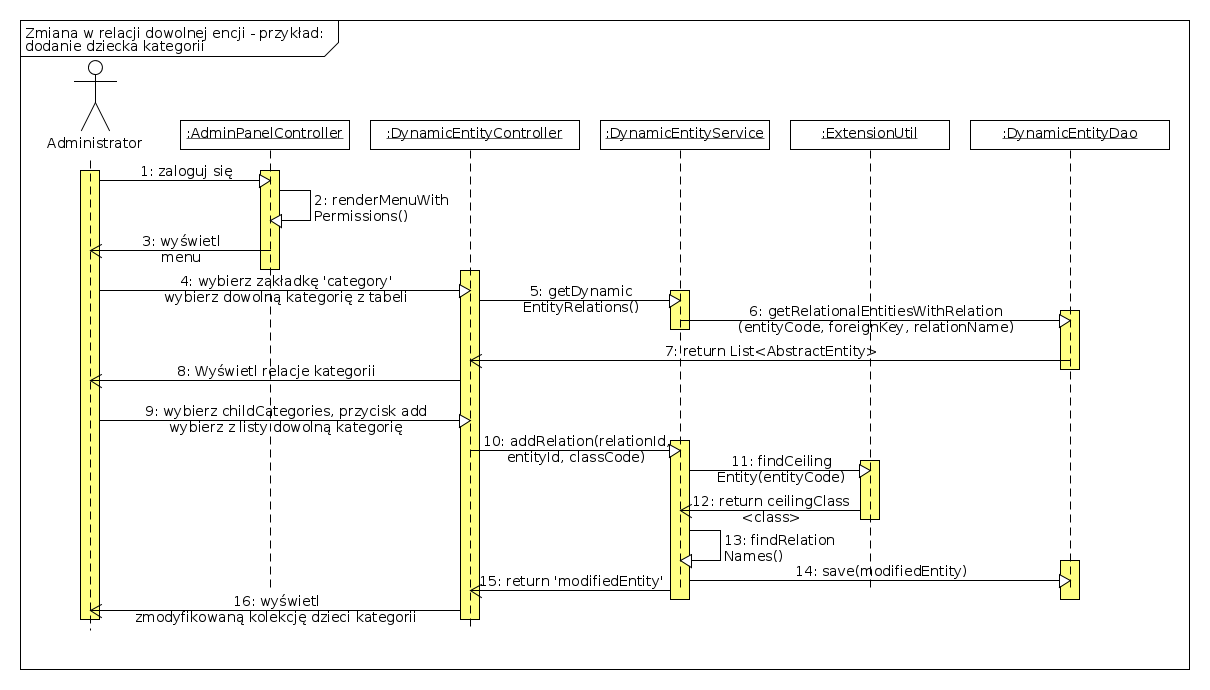
\includegraphics[scale=0.4]{zmianaWRel.png}
 	\end{center}
 	\caption{{\color{black}Diagram sekwencji opisujący opisujący zmianę właściwości dowolnej encji na przykładzie produktu.}} \label{zmianaWRel}
 \end{figure}

\subsection{Dodanie dowolnej encji na przykładzie atrybutu klasyfikacyjnego}
Ta ważna część frameworku zostanie przedstawiona na podstawie dodawania facetu - czyli atrybutu, po którym można filtrować produkt. Tak jak w powyższych sekcjach, nie ma dużego znaczenia jaką encję dodajemy - generyczny formularz i mechanizm uzupełniania pól w obiekcie danej klasy jest taki sam dla wszystkich encji w systemie. Dzięki diagramowi sekwencji z rysunku \ref{dodanieFacetu} można zobaczyć jak dodać atrybut do produktu, który będzie możliwy do wyszukania w sklepie, a zarazem zobaczyć jak w systemie utrwalane są nowe obiekty. Tym razem refleksja została użyta do przepisania wartości z formularza do obiektu (punkty 8 do 12) oraz do znalezienia najwyższej w hierarchii klasy modyfikowanej encji (pkt 5). 

Jak zostało już wspomniane, każdy atrybut może mieć wartości, które powinien przyjmować, np. \textit{rodzaj podszewki: skórzana/gumowa/materiałowa}. Dlatego do atrybutu klasyfikacyjnego możliwe jest zdefiniowane jego przyjmowanych wartości, dzieje się to w dokładnie ten sam sposób, jak na rysunku \ref{dodanieFacetu}, jedynie encja \texttt{CategoryFeature} (atrybut klasyfikacyjny) zmienia się na \texttt{Category-} \texttt{FeatureValue}. Po dodaniu możliwych wartości dla stworzonego atrybutu, należy je do niego przypisać w sposób opisany na diagramie z rysunku \ref{zmianaWRel}. W ten sam sposób przypiszemy również stworzony atrybut do kategorii. Zostanie on uwzględniony w wynikach wyszukiwania opisanych w podrozdziale \textbf{Wyszukiwanie produktu}. Aby rozjaśnić rozważania, został przytoczony przykład \ref{przyklAtrubyt}.
\begin{example} 
	Załóżmy, że w mamy kategorię obuwie, chcielibyśmy aby każdy produkt w wynikach wyszukiwania w sklepie był możliwy do odfiltrowania na podstawie rodzaju podszewki. W tym celu dodajemy atrybut klasyfikacyjny Podszewka z zaznaczeniem, że ma być to facet (filtr). Dodajemy 3 wartości: skórzana/gumowa/materiałowa. Przypisujemy możliwe wartości do atrybutu, sam atrybut do kategorii obuwie, od tej pory w formularzu edycyjnym produktu, który znajdzie się w kategorii obuwie, znajdziemy pole rodzaj podszewki. Co więcej gdy więcej niż jeden znaleziony przy wyszukiwaniu w sklepie produkt będzie miał zdefiniowany dla siebie ten atrybut, to pojawi się on (atrybut) jako przycisk do odfiltrowania wyników wyszukiwania.  
	\label{przyklAtrubyt}
\end{example}
 
  \begin{figure}
 	\begin{center}
 		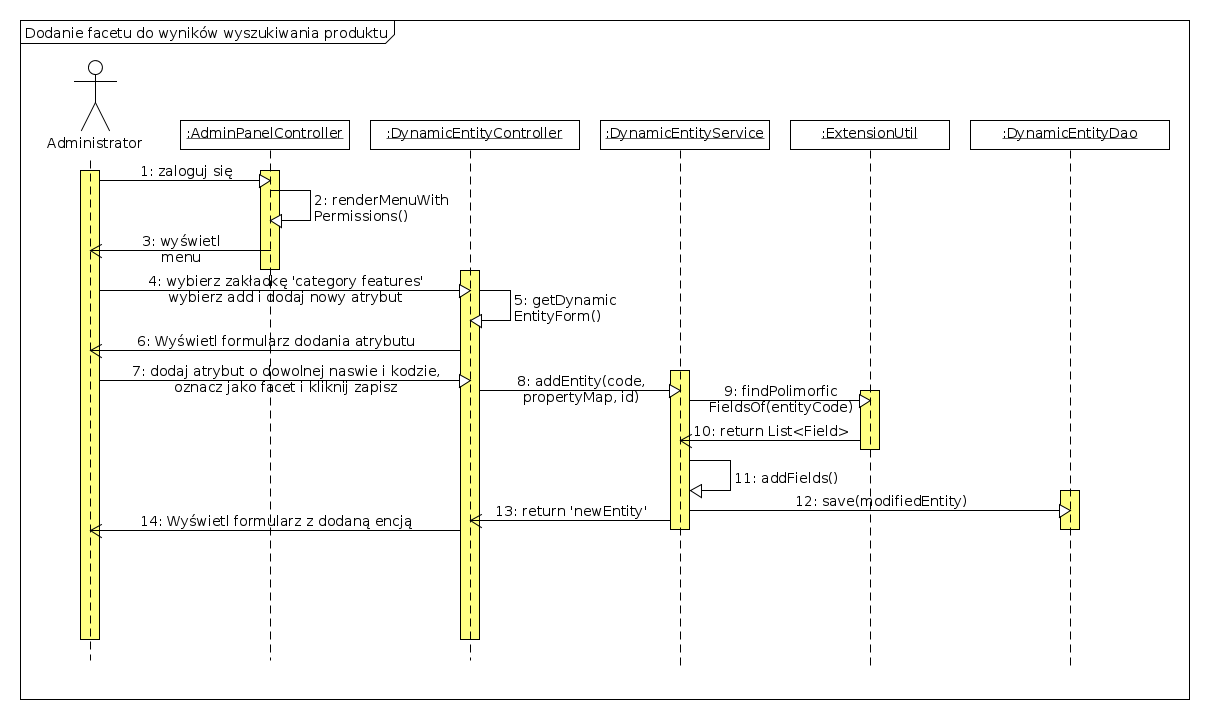
\includegraphics[scale=0.38]{dodanieFacetu.png}
 	\end{center}
 	\caption{{\color{black}Diagram sekwencji opisujący dodanie dowolnej encji na przykładzie atrybutu klasyfikacyjnego.}} \label{dodanieFacetu}
 \end{figure}

\subsection{Wyszukiwanie produktu}
Proces wyszukiwania produktu został ujęty na diagramie z rysunku \ref{wyszukiwanieProdSekw}. Aby przedstawić to jak najbardziej obrazowo, w procesie uczestniczą trzy komponenty: frameworkowy kontroler wyszukiwania, serwer Solr, który przechowuje produkty w płaskiej strukturze i baza danych relacyjna, która przechowuje pola i włąsciwości produktu podlegające mechnizmowi wyszukiwania. Na początku z bazy danych wciągane są właściwości i wszystkie zmienne, czyli to czy dane pole ma być wyszukiwane tekstowo, czy ma być filtrem (facetem). Następnie budowana jest dynamiczna kwerenda i wysyłana na serwer Apache Solr, który zwraca wyniki przetwarzane w punktach 10 do 12. Tworzone są wtedy reprezentacje filtrów jak i samych wyników wyszukiwania, czyli produktów. 

Wart zauważenia jest region \textit{cached} w ramce, otóż jednym z postulatów frameworku było nie korzystanie z bazy danych relacyjnej przy wyszukiwaniu w katalogu produktowym (najbardziej obciążony fragment systemu), dlatego właściwości potrzebne do stworzenia kwerendy są pobierane raz, a później trzymane w pamięci cache (jest to mechanizm domyślnie dostarczany przez Hibernate, nie wymagał on implementacji). 
  \begin{figure}
	\begin{center}
		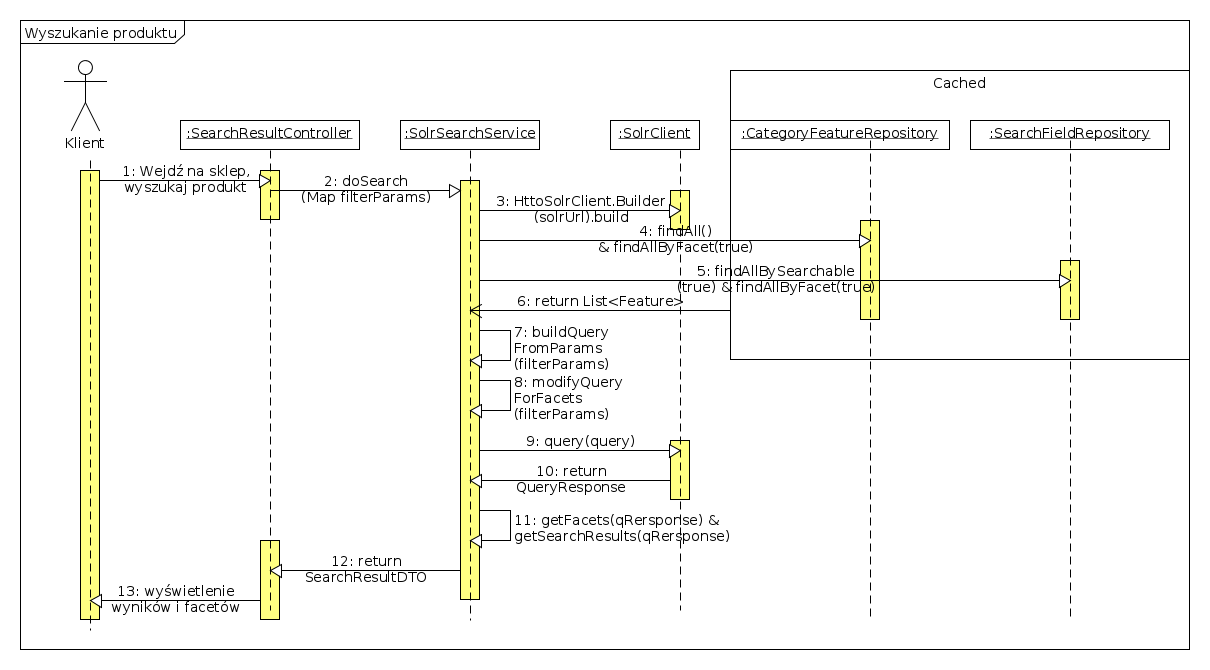
\includegraphics[scale=0.38]{wyszukanieProdSekw.png}
	\end{center}
	\caption{{\color{black}Diagram sekwencji opisujący proces wyszukiwania produktu.}} \label{wyszukiwanieProdSekw}
\end{figure}



\subsection{Proces zakupowy}
Proces zakupowy jest standardowym mechanizmem konicznym do przeprowadzenia transakcji, nie wymaga on szczególnej optymalizacji, ze względu na to, że nie jest to obciążona część platformy. Klient końcowy, po wejściu na sklep może wyszukać produkt oraz zdefiniować kryteria wyszukiwania. Po znalezieniu szukanych produktów może umieścić je w koszyku, a następnie zamówić elementy dodane do koszyka. Szczególnym rozwiązaniem dla frameworka jest tworzenie kopii produktu w momencie składania zamówienia, aby klient w razie reklamacji miał się do czego odwołać. Ta funkcjonalność, jest umotywowana tym, że cechy produktu w systemie są bardzo dynamiczne i mogą być dowolnie zmieniane, więc produkt sprzedany w danym miesiącu może być niemożliwy do odnalezienia po pewnym czasie. Całość została umieszczona na diagramie z rysunku \ref{procZakup}.
\begin{figure}
	\begin{center}
	%	\includegraphics[scale=0.4]{procZakup.png}
	\end{center}
	\caption{{\color{black}Diagram sekwencji opisujący proces zakupowy.}} \label{procZakup}
\end{figure}


\newpage
\section{Diagramy klas}

Na podstawie wcześniejszych rozważań możliwe jest zdefiniowanie następujących części frameworku: 
\begin{itemize}
	\item części przewidziane dla programisty i administratora sklepu
	\subitem konfigurowalne menu w panelu administracyjnym
	\subitem dynamiczny formularz encyjny
	\subitem dynamiczna tabela encyjna
	\item części przewidziane dla administratora sklepu
	\subitem system klasyfikacyjny
	\subitem struktura uprawnień w panelu administracyjnym
	\subitem mechanizm indeksacji i wyszukiwania produktów
	\item część przewidziana dla użytkownika końcowego - klienta sklepu
	\subitem mechanizm wyszukiwania produktów
	\subitem proces zamówienia i archiwizacji produktu
\end{itemize}
Diagramy klas zostaną podzielone ze względu na pochodzenie funkcjonalności zdefiniowane wyżej. 

%\subsection{System klasyfikacyjny i katalog produktowy}

\subsection{Konfigurowalne menu}
Na diagramie \ref{klasy_menu} został przedstawiony diagram klas dla menu panelu administracyjnego. Aby zapewnić możliwość obsługi dowolnej encji w panelu administracyjnym, które zostały zaimplementowane na potrzeby sklepu, np. Order (zamówienie), zostało stworzone menu, które jest oparte na klasie AdminMenuItem. Klasa ta bespośrednio odpowiada dowolnej encji. Oznacza to, że jeśli encja powinna być obsługiwana z panelu administracyjnego, to musi w systemie (jego bazie danych) istnieć jej odpowiednik w postaci rekordu AdminMenuItem z nazwą jej klasy (\texttt{className}). W systemie została przewidziana możliwość grupowania poszczególnych zakładek za pomocą klasy \texttt{AdminMenuGroup}. Budowanie menu odbywa się w klasie \texttt{DynamicEntityController}, która korzysta z klas połączonych z bazą danych, tak aby móc zaczytywać kolejne encje (\texttt{AdminMenuGroupRepository i AdminMenuItemRepository}). Dla lepszego zrozumienia został podany przykład \ref{przyklad_menu}
\begin{example}
	W systemie istnieje encja Order, chcielibyśmy mieć możliwość zarządzania tą encją z poziomu panelu administracyjnego. W tym celu na poziomie bazy danych powinna być zapisany egzemplarz AdminMenuItem z nazwą klasy (className): com.example.model.Order (nazwa pakietu została podana tylko dla przykładu). System w tym momencie rozpozna encję Order, wyświetli ją w menu oraz będzie w stanie stworzyć dla niej tabele encyjną ze wszystkimi rekordami oraz formularz edycji. 
\end{example} 
\begin{figure}
	\begin{center}
		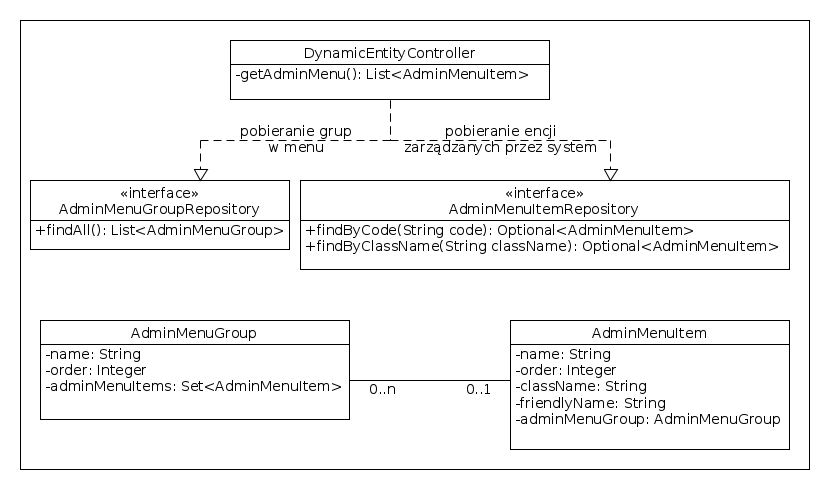
\includegraphics[scale=0.5]{klasy_menu.png}
	\end{center}
	\caption{{\color{black}Diagram klas dla menu w panelu administracyjnym}} \label{klasy_menu}
\end{figure}

\subsection{Dynamiczna tabela encyjna}
Na rysunku \ref{klasy_tabela_encyjna} został umieszczony diagram klas dla dynamicznej tabeli encyjnej, o której była mowa w poprzedniej podsekcji. Tabela ta służy do wyświetlania wszystkich egzemplarzy danej encji w systemie, np. wszystkie produkty lub kategorie. Aby zamodelować tabelę zostały zaimplementowane dwie klasy: \texttt{DynamicEntityTable i AbstractTableLine}. Odpowiednio odpowiadają one całej strukturze tabeli oraz pojedynczemu wierszowi. Oczywisty jest fakt, że tabela musi posiadać wiele wierszy. \texttt{DynamicEntityService} używa tych klas do konstrukcji tabelki. Serwis musi mieć możliwość pobierania danych z bazy, jednak jest to utrudnione zadanie ze względu na to, że nie jest z góry określone, że akurat ten serwis zawsze konstruuje tabelkę klasy, np. \texttt{Product}. W tym celu została zaimplementowana klasa \texttt{DynamicEntityDao}. Jest to obiekt typu DAO\footnote{DAO - Data Access Object - obiekt dostępu do bazy danych}, którego zadaniem jest wyciągać z bazy danych encje zdefiniowane w systemie (te obecne w bazie danych jako egzemplarze klasy \texttt{AdminMenuItem}), niezależnie od tego jakiej klasy są i czy nie zostały nadpisane. Stąd metoda \texttt{getCeilingClass(className)}, która odpowiada za znalezienie \textit{najmłodszej} klasy w abstrakcji. Aby rozjaśnić ten mechanizm został podany przykład \ref{przyklad_tabela}
\begin{example}
\label{przyklad_tabela}
	W systemie istnieje wiele encji, np. Customer, Order, Product. W przypadku generowania dla nich tabeli, należy pamiętać o tym, że każda z nich może zostać nadpisana przez programistów budujących rozwiązania oparte o implementowany framework. Powiedzmy, że dodano klasę \texttt{MyProduct extends Product}. Abyśmy otrzymali dostęp do pól z tej nowej, nieznanej systemowi klasy potrzebujemy właśnie metody, która znajdzie za pomocą refleksji klasę \texttt{MyProduct}, dzięki której system automatycznie, bez wkładu programisty będzie mógł uwzględnić w tabeli encyjnej pola, które zostały dopisane do produktu. To jest właśnie zadanie metody \texttt{getCeilingClass}. 
\end{example}
Kontroler \texttt{DynamicEntityControler} korzysta z serwisu, aby umieścić tabelę z encjami na stronie panelu administracyjnego pod konkretnym mapowaniem, np. \textit{/admin/entity/product/table}. 
\begin{figure}
	\begin{center}
		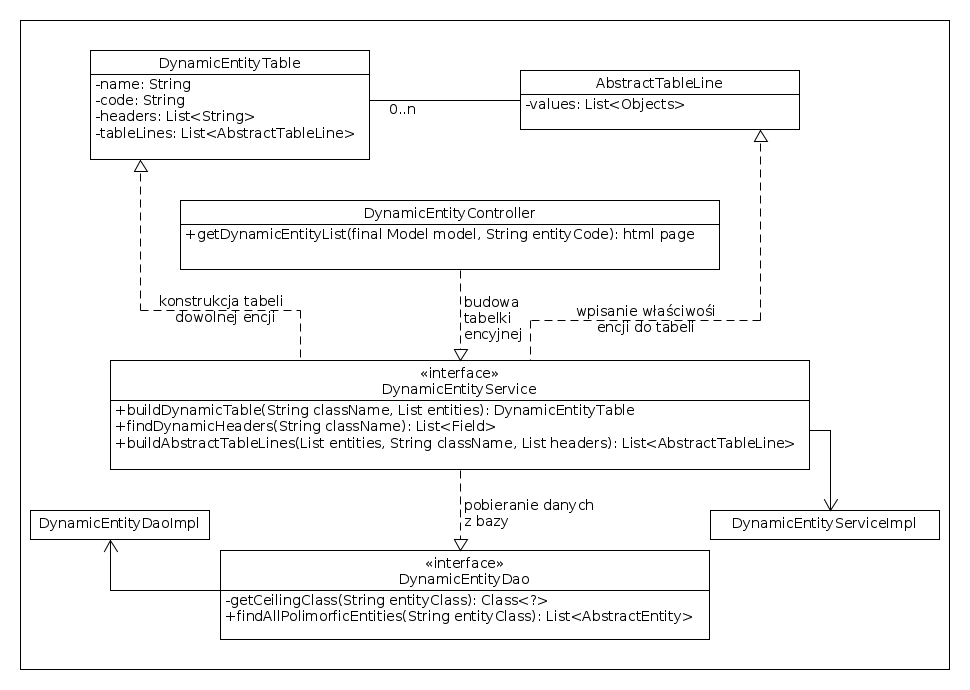
\includegraphics[scale=0.4]{klasy_tabela_encyjna.png}
	\end{center}
	\caption{{\color{black}Diagram klas dla tabeli encyjnej w panelu administracyjnym}} \label{klasy_tabela_encyjna}
\end{figure}

\subsection{Dynamiczny formularz encyjny}
Na rysunku \ref{klasy_formularz_encyjny} został umieszczony diagram klas dla dynamicznego formularza edycji encji. Zdefiniowano dla niego dwa rodzaje pól: \texttt{DynamicFormField i RelationMetadata}. Odpowiadają one odpowiednio polom prostym oraz relacyjnym. Każde pole relacyjne ma tabelkę z encjami (\texttt{DynamicEntityTable} - modelowo jest to ta sama tabelka co w poprzedniej podsekcji) będącymi w relacji z encją dla której generowany jest formularz, np. kolekcja cen w każdym produkcie. Dynamiczny serwis encyjny podobnie jak w przypadku tabeli, konstruuje formularz korzystając z opisanych wyżej modelowych klas. Posiada zestaw metod które:
\begin{itemize}
	\item wyciągają wartości pól z encji za pomocą refleksji (tak eby wpisać je do formularza edycji)
	\item znajdują za pomocą refleksji relacje encji, dla której budowany jest formularz, z uwzględnieniem problemu nadpisanej klasy opisanego w przykładzie \ref{przyklad_tabela}
	\item obsługują CRUD edytowanej encji oraz jej relacji 
\end{itemize}  

\texttt{DynamicEntityController} w przypadku tej funkcjonalności obsługuje zapytania z serwera związane z wyświetleniem formularza encji, przetwarzaniem edycji oraz obsługą relacji encji (CRUD\footnote{CRUD - CreateReadUpdateDelete - zestaw podstawowych operacji na encji, w przypadku tej funkcjonalności odnosi się do obsługi pól relacyjnych w encji, np. dodawania, usuwania, czytania i edytowania zdjęć do produktu }). Klasa \texttt{DynamicEntityDao} spełnia takie samo zadanie jak w przypadku tabeli -- wyciąga z bazy danych egzemplarze encji z uwzględnieniem możliwej abstrakcji.
\begin{figure}
	\begin{center}
		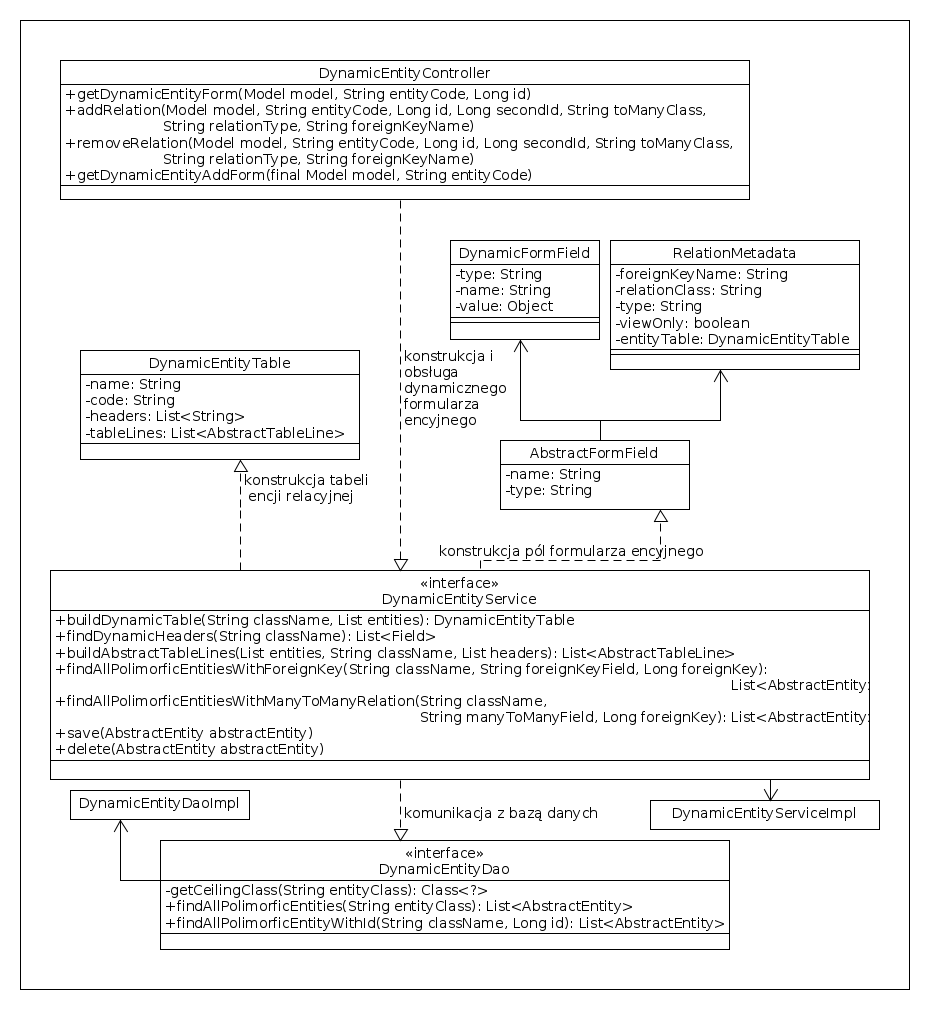
\includegraphics[scale=0.4]{klasy_formularz_encyjny.png}
	\end{center}
	\caption{{\color{black}Diagram klas dla tabeli encyjnej w panelu administracyjnym}} \label{klasy_formularz_encyjny}
\end{figure}

\subsection{Model systemu klasyfikacyjnego}
System klasyfikacyjny jest powiązany z drzewem kategorii. Pozwala na zdefiniowanie dziedzicznych cech dla każdej z nich, które pojawią się w końcowym produkcie przypisanym do kategorii. Poniżej znajduje się opis słowny poszczególnych klas ujętych na diagramie \ref{klasy_model_sysKlas}.

\noindent Cechy kategorii (\texttt{com.tinecommerce.core.catalog.model::Category}):
\begin{itemize}
	\item dowolna liczbę dzieci i rodziców
	\item lista asocjacji do zdefiniowanych jej cech
	\item przypisane do niej produkty
\end{itemize} 
Cechy produktu (\texttt{com.tinecommerce.core.catalog.model::Product}):
\begin{itemize}
	\item lista cen
	\item lista przypisanych kategorii
	\item lista cech (ProductFeature)
\end{itemize}
\texttt{Product Feature} jest to klasa pośrednicząca pomiędzy strukturą drzewiastą systemu klasyfikacyjnego, a samym produktem, dlatego jej cechy to: produkt, cecha kategorii oraz jej wartość. Warto zauważyć, że z punktu widzenia modelu jest możliwe aby każdy produkt posiadał dowolną cechę wynikającą z klasyfikacji, ponieważ Product i CategoryFeature są  \textit{de facto} w relacji many to many. Jednak warstwa serwisowa (opisana w dalszej sekcji) jest odpowiedzialna za ograniczenie tych cech tylko do takich, które wynikają ze ścieżki w drzewie kategorii, która prowadzi od korzenia do samego produktu. Aby jaśniej nakreślić udział modelu w systemie klasyfikacyjnym został podany przykład \ref{przyklCatFeat}
\begin{example}
	\label{przyklCatFeat}
	Kategoria (Category) \textbf{sport} posiada atrybut klasyfikacyjny (Category Feature) \textbf{waga sprzętu}, ich powiązanie definiuje się encją Category Feature Assignment. Atrybut klasyfikacyjny może mieć zdefiniowane wiele możliwych dla siebie wartości (Category Feature Value), np. \textbf{5KG, 2KG, 1KG}. Jeżeli jakiś produkt będzie należał do kategorii \textbf{sport}, to w jego fromularzu edycji pojawi się możliwe do zdefiniowania pole (Product Feature) \textbf{waga sprzętu}, której będziemy mogli nadać wartość \textbf{5KG, 2KG, 1KG}.
\end{example}

\begin{figure}
	\begin{center}
		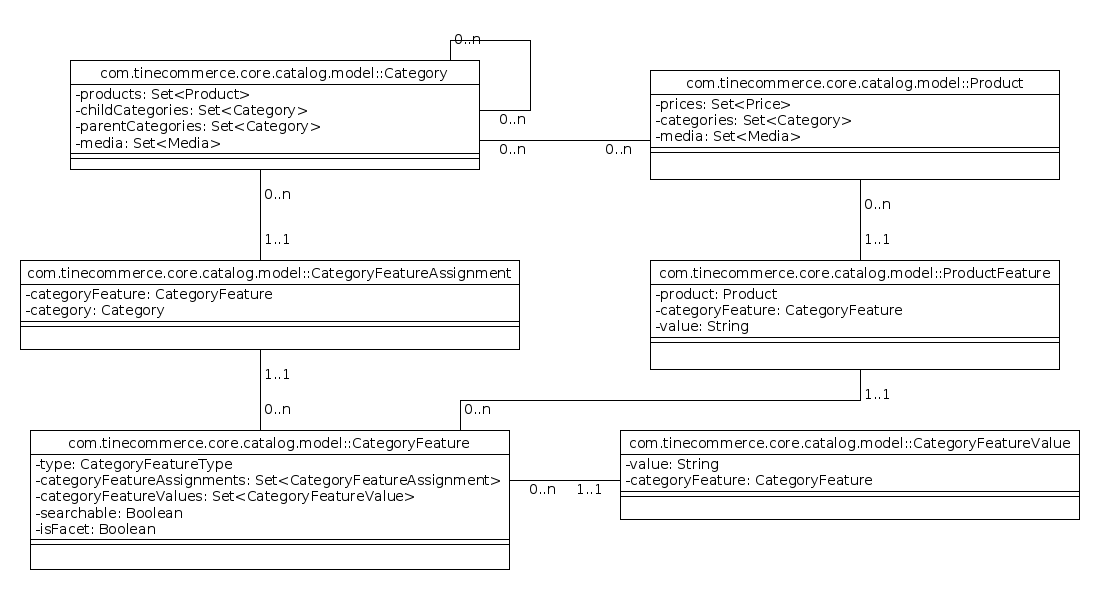
\includegraphics[scale=0.4]{klasy_model_sysKlas.png}
	\end{center}
	\caption{{\color{black}Diagram klas systemu klasyfikacyjnego - model}} \label{klasy_model_sysKlas}
\end{figure}

\subsection{Warstwa serwisowa systemu klasyfikacyjnego}
Na rysunku \ref{klasy_serwisy_sysKlas} został umieszczony diagram klas warstwy serwisowej systemu klasyfikacyjnego. W opisie modelu zostało wspomniane, że warstwa serwisowa zajmuje się ograniczeniem atrybutów klasyfikacyjnych i przypisywaniem ich produktom. Ponadto zapewnia walidacje drzewa kategorii (aby nie powstawały cykle).

\noindent
\textbf{Serwis kategorii} (CategoryService) jest interfejsem, który waliduje strukture drzewa kategorii, dodaje kategorie do drzewa (tworzy powiazania) oraz umożliwia wydobycie wszystkich przodków i potomków węzła. Serwis w przypadku znalezienia cyklu w drzewie kategorii rzuca wyjątek informujący o cyklicznym połączeniu między kategoriami (CircularEntityConnectionException) Interfejs posiada podstawową implementację w postaci klasy CategoryServiceImpl. 

\noindent
\textbf{Serwis atrybutów klasyfikacyjnych} (CategoryFeatureService) został zaimplementowany po to aby umożliwić pobranie wszystkich możliwych atrybutów klasyfikacyjnych dla dowolnego Produktu. To właśnie ten serwis jest odpowiedzialny za ograniczenie tych cech tylko do takich, które wynikają ze ścieżki w drzewie kategorii, która prowadzi od korzenia do samego produktu. Sytuacja ta została opisana na diagramach aktywności w sekcji \textbf{Wyszukiwanie cech produktu}.

Serwisy mają również połączenie z bazą danych za pomocą obiektów \textit{repository}. W tych klasach są konkretne metody pobierające encje z bazy danych. Każda metoda odpowiada kwerendzie bazodanowej, która została wygenerowana przez framework Hibernate na podstawie nazwy metody. 
\begin{figure}
	\begin{center}
		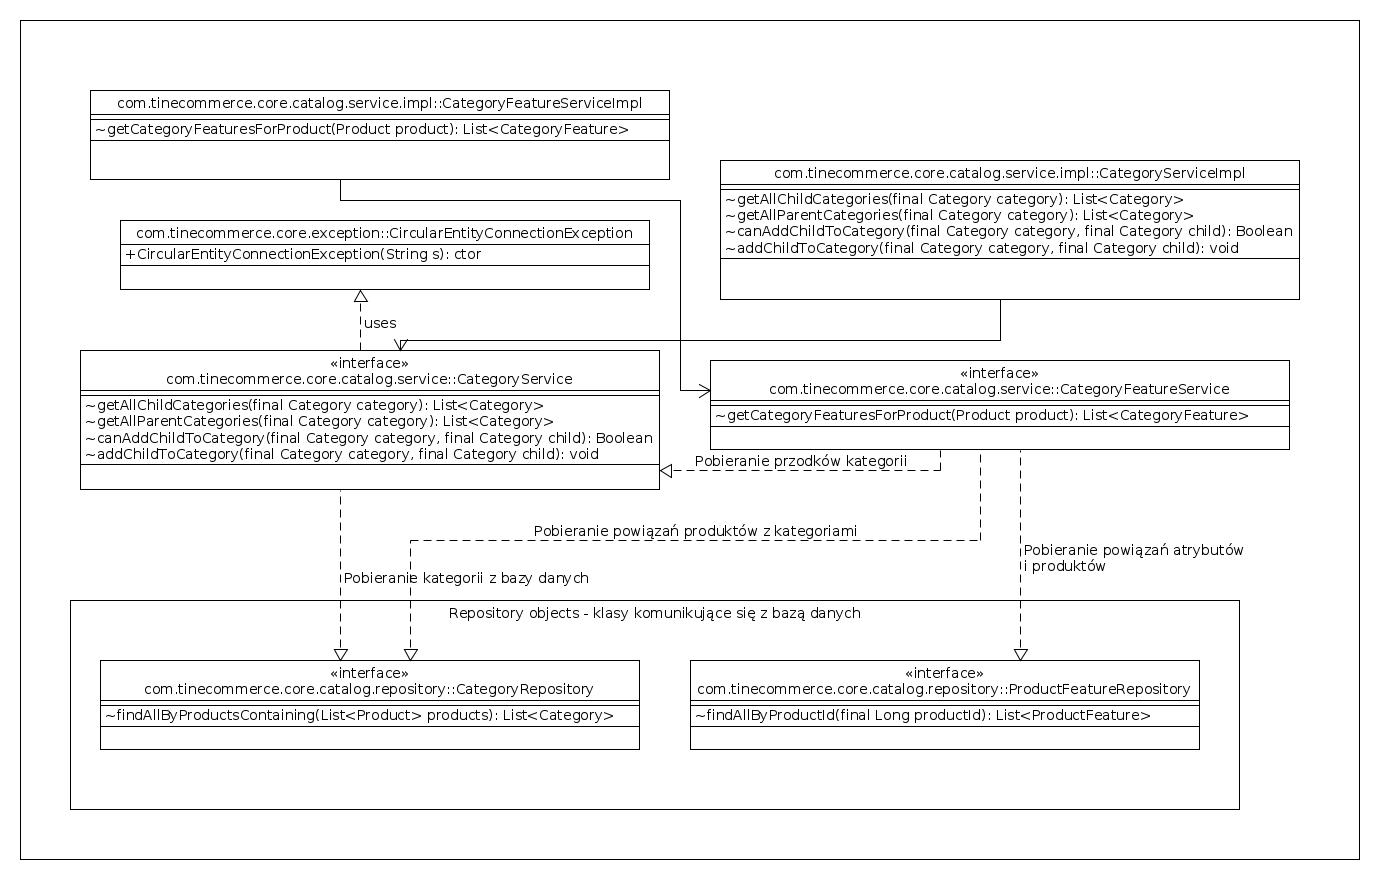
\includegraphics[scale=0.38]{klasy_serwisy_sysKlas.png}
	\end{center}
	\caption{{\color{black}Diagram klas systemu klasyfikacyjnego - serwisy}} \label{klasy_serwisy_sysKlas}
\end{figure}

\subsection{Warstwa kontrolerów systemu klasyfikacyjnego}
Rysunek \ref{klasy_kontrolery_sysKlas} przedstawia diagram klas warstwy kontrolerów systemu klasyfikacyjnego. Panel administracyjny i edycja encji w systemie jest oparta na refleksji (czyli wyciąganiu wartości pól z klas), jednak w przypadku atrybutów klasyfikacyjnych nie mamy do czynienia z fizycznymi polami, dlatego potrzebujemy mechanizmu, który obsłuży przypisywanie im wartości, dodawanie ich lub usuwanie. Kontrolery związane z systemem klasyfikacyjnym są rozszerzeniem ogólnego \textbf{DynamicEntityController} (omówionego w poprzednich sekcjach), który zapewnia właśnie domyślne rozwiązanie oparte na refleksji. Więc powstały one ze względu na konieczność obsługi nietypowych pól w formularzu edycji produktu jak i kategorii. W przypadku produktu są to pola, które nie należą bezpośrednio do klasy Product, jednak mogą mieć zdefiniowaną wartość - czyli wartości atrybutów klasyfikacyjnych. Natomiast w przypadku kategorii wiąże się to z koniecznością walidacji dodawania kolejnych powiązań w drzewie kategorii. 
\begin{figure}
	\begin{center}
		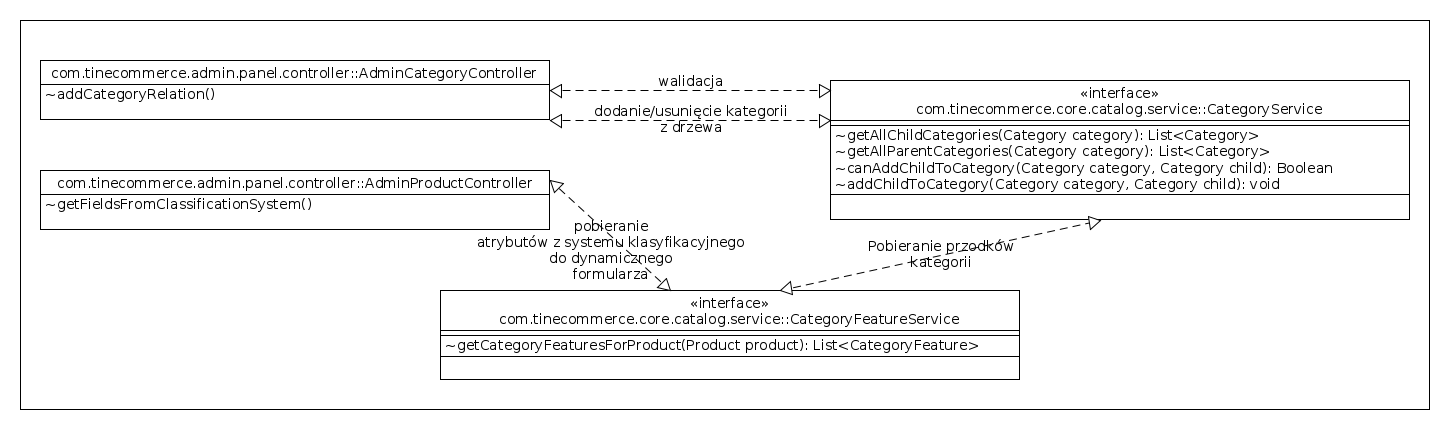
\includegraphics[scale=0.4]{klasy_kontrolery_sysKlas.png}
	\end{center}
	\caption{{\color{black}Diagram klas systemu klasyfikacyjnego - kontrolery}} \label{klasy_kontrolery_sysKlas}
\end{figure}

\subsection{Struktura uprawnień w panelu administracyjnym}
Panel administracyjny wyposażony jest w drzewiasty system uprawnień, który zapewnia kontrole dostępu do encji dla różnych użytkowników. Diagram klas użytych w tym rozwiązaniu został przedstawiony na rysunku \ref{klasy_uprawnienia}. \texttt{DynamicEntityControler} w przypadku tej funkcjonalności sprawdza w swoich metodach CRUD dotyczących encji, czy zalogowany użytkownik ma prawo do wyświetlenia i edycji encji, w którą ma zamiar wejść. Dzieje się to za sprawą metody \texttt{hasPermissionForOperation}
\texttt{(className)} w klasie \texttt{AdminPermissionService}, która wędrując po drzewie uprawnień sprawdza czy dany użytkownik ma powiązanie z uprawnieniem potrzebnym do wyświetlenia danej encji. Obiekty z bazy danych są pobierane za pomocą klasy \texttt{AdminUserRepository}. System skonfigurowany jest domyślnie na to aby jeden egzemplarz klasy \texttt{AdminPermission} odpowiadał jednej klasie encyjnej (np. cenie - Price). Uprawnienia mają również listę dzieci, dlatego można je układać w drzewiaste struktury. Działąnie struktury objaśni przykład \ref{przyklad_upraw}
\begin{example}
	\label{przyklad_upraw}
	Gdy użytkownik administracyjny \texttt{AdminUser} otrzymuje dane uprawnienie A, jest w stanie wyświetlić i edytować encję, której dotyczy to uprawnienie A jak i również wszystkie inne encje, których dotyczą uprawnienia, dla których A jest rodzicem. 
\end{example}
\begin{figure}
	\begin{center}
		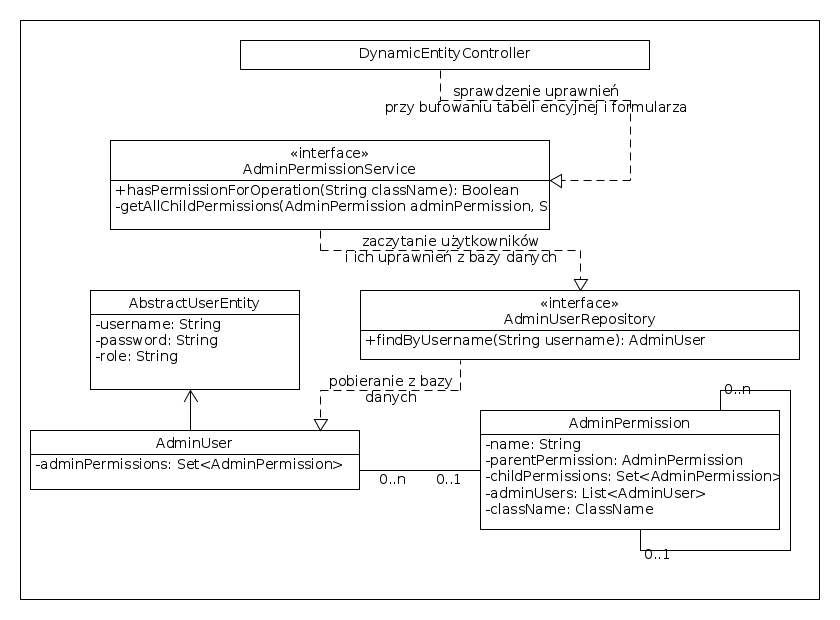
\includegraphics[scale=0.4]{klasy_uprawnienia.png}
	\end{center}
	\caption{{\color{black}Diagram klas systemu uprawnień}} \label{klasy_uprawnienia}
\end{figure}

\subsection{Indeksacja i wyszukiwanie produktów}
W systemie zostały zaimplementowane dwa główne serwisy obsługujące zapytania związane z wyszukiwaniem i widzialnością produktów na sklepie. Pierwszy z nich to \texttt{SolrIndexService}, którego zadaniem jest wydobyć atrybuty produktu z systemu klasyfikacyjnego oraz z pól jego klasy jak zostało to przedstawione na rysunku \ref{cechyProd}. Potrzebuje on w tym celu dwóch obiektów dostępów do bazy dancyh. \texttt{ProductRepository} wyciągnie produkty (\texttt{Product}) wraz z kolekcjami ich dynamicznych cech z systemu klasyfikacyjnego (\texttt{ProductFeature/CategoryFeature}). Natomiast \texttt{SearchFieldRepository} wyciągnie nazwy pól, które zosatły zdefiniowane w systemie jako potrzebne do indeksacji (np. nazwa, opis lub cena). Każdy egzemplarz klasy \texttt{SearchField} odpowiada więc pewnej cesze produktu, która ma być wyszukiwalna. Cechy te zostaną wyciągnięte z klasy \texttt{Product} i jego ewentualnych nadklas (np. opisywany wielokrotnie hipotetyczny \textit{MyProduct}). Wszystkie atrybuty produktu są pakowane w tak zwane \textit{dokumenty} (jeden dokument odpowiada jednemu produktowi) i wysyłane na serwer Apache Solr. Zaindeksowany Solr jest wtedy gotowy do przyjmowania zapytań dotyczących wyszukiwania. \textbf{SolrSearchService} jest odpowiedzialny za konstruowanie kwerend Solrowych i interpretacje wyników wyszukiwania.
\begin{figure}
	\begin{center}
		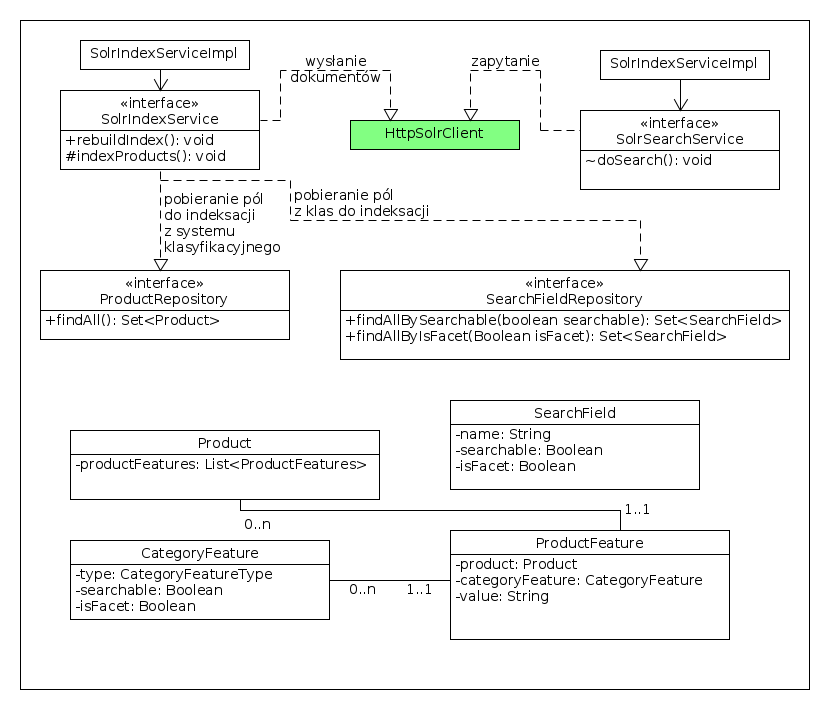
\includegraphics[scale=0.4]{klasy_solr.png}
	\end{center}
	\caption{{\color{black}Diagram klas mechanizmu indeksująco-wyszukującego}} \label{klasy_solr}
\end{figure}

\subsection{Proces zamówienia}
Jeden z najbardziej charakterystycznych procesów we frameworku e-commerce to proces zamówienia, diagram klas użytych do implementacji tego procesu został umieszczony na rysunku \ref{klasy_koszyk}. \texttt{CartController} odpowiada za obsługę zapytań związanych z operacjami na koszyku takimi jak dodawanie, usuwanie, złożenie zamówienia, wyświetlenie koszyka. Serwis zamówień \texttt{OrderService} obsługuje logikę tych zapytań wraz z funkcjonalnością archiwizacji cech produktu (metoda \texttt{archvizePr-} \texttt{oduct(Product product)}). Serwis używa singletonów Repository, aby znajdować w bazie danych zamówienia rozpoczęte przez zalogowanych użytkowników, produkty i szczegóły kupujących. 
\begin{figure}
	\begin{center}
		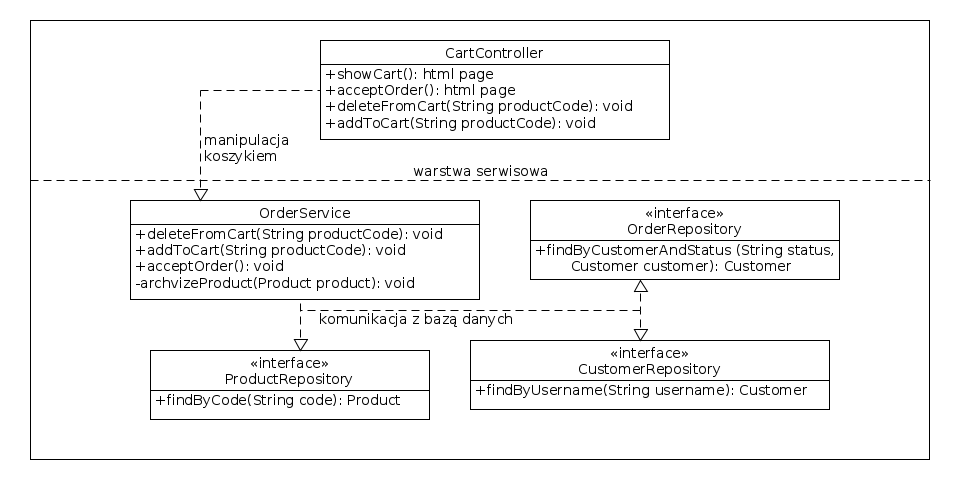
\includegraphics[scale=0.4]{klasy_koszyk.png}
	\end{center}
	\caption{{\color{black}Diagram klas procesu zamówienia}} \label{klasy_koszyk}
\end{figure}

\newpage
\section{Projekt bazy danych}
W tej sekcji został przedstawiony projekt bazy danych. Dla zachowania ciągłości i przejrzystości rozważań diagramy zostały podzielone ze względu na funkcjonalności, podobnie jak na diagramach klas: 
\begin{itemize}
	\item menu w panelu administracyjnym
	\item system klasyfikacyjny
	\item struktura uprawnień
	\item proces zamówienia i archiwizacji produktu
\end{itemize}
Następnie w podsekcji \textbf{Mechanizm wyszukiwania} została opisana nierelacyjna baza Apache Solr i jej korelacje z relacyjną bazą danych. Na samym końcu została omówiona platforma DBMS i normalizacja relacyjnej części bazy danych.

Warto zaznaczyć w tym miejscu, że większość tabel ma kod (\texttt{code}), który jest unikalnym kluczem, po którym (zaraz obok id) można wyciągać encje z tabeli. Takie rozwiązanie zwiększa bezpieczeństwo aplikacji webowej, gdyż na stronie sklepu dostępnej dla osób trzecich nie są ujawniane klucze główne, tylko kody, które jednoznacznie określają encję w tabeli. Pogrubione kolumny w tabelach oznaczają unikalność wartości. 

\subsection{Menu w panelu administracyjnym}
Na rysunku \ref{db_menu} został umieszczony diagram fragmentu bazy danych odpowiadający za menu w panelu. Zostało ono oparte na dwóch tabelach relacyjnych \texttt{admin\_menu\_item} (zakładka w menu) oraz \texttt{admin\_menu\_group} (grupa zakładek). Do pierwszej z nich składa się z id, unikalnego kodu, nazwy klasy, jaką ma reprezentować dana zakładka, kolejności wyświetlania, nazwy i nazwy wyświetlanej (\texttt{friendly\_name}) oraz \texttt{group\_id}, czyli klucza obcy grupy, w której się znajduje. Te dwie tabele łączy relacja one to many, w której rodzicem jest \texttt{admin\_menu\_group}. Nie jest konieczne aby grupa musiała zawierać jakiekolwiek elementy, podobnie nie jest obligatoryjne aby element musiał być przypisany do konkretnej grupy. 

\begin{figure}
	\begin{center}
		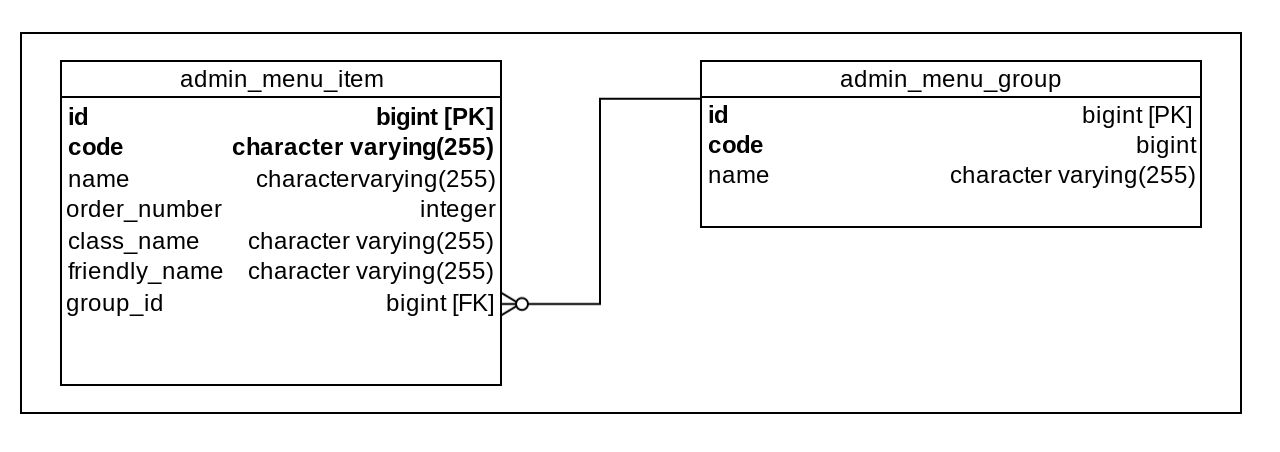
\includegraphics[scale=0.3]{db_menu.png}
	\end{center}
	\caption{{\color{black}Diagram fragmentu bazy danych odpowiadającego za menu}} \label{db_menu}
\end{figure}

\subsection{System klasyfikacyjny}
Diagram na rysunku \ref{db_sysKlas} przedstawia część bazy danych odpowiadającą za system klasyfikacyjny. Ze względu na obszerność diagramu, tabele zostaną omówione jedna po drugiej. 
\begin{itemize}
	\item \texttt{category} -- główna tabela zawierająca kategorię produktów dostępnych w systemie, kategorie mogą przyjmować strukturę drzewa, w którym każdy węzeł ma dowolną ilość dzieci i rodziców, dlatego tabela jest w relacji many to many ze samą sobą. 
	\item \texttt{product} -- tabela przechowująca produkty dostępne w systemie, powiązana relacją many to many z kategoriami, tym sposobem każdy produkt może być w dowolnie wielu kategoriach oraz każda kategoria może być przypisana do wielu produktów. 
	\item \texttt{category\_feature} -- w tej tabeli przechowuje się atrybuty klasyfikacyjne, które mogą zostać przypisane do kategorii, oprócz standardowych kolumn takich jak nazwa lub opis, są również flagi, które informują system o tym czy dany atrybut ma być wyszukiwalny pełnotekstowo na sklepie (\texttt{searchable}) lub czy ma być filtrem ograniczającym wyniki wyszukiwania (\texttt{is\_facet}). Tabela ta jest w relacji many to many z tabelą \texttt{category}, co umożliwia kategorii mieć wiele atrybutów i atrybutowi znaleźć się w wielu kategoriach.
	\item \texttt{category\_feature\_assignment} -- jest to tabela asocjacyjna pomiędzy kategorią, a atrybutem klasyfikacyjnym. Posiada ona własne id i kod, gdyż jest również systemową encją.
	\item \texttt{category\_feature\_value} -- każdy atrybut klasyfikacyjny może mieć predefiniowane wartości, które składowane są w tej tabeli. \texttt{category\_feature\_value} jest powiązane relacją one to many z \texttt{category\_feature} z kluczem obcym \texttt{category\_feature\_id}.
	\item \texttt{product\_feature} -- jest to tabela, która pozwala na powiązanie produktu atrybutami klasyfikacyjnymi jest w relacji one to many z tabelą \texttt{product i category\_feature}, ma w tym celu dwa klucze obce  \texttt{category\_feature\_id} i  \texttt{product\_id}. Pozwala również przypisać wartość atrybutowi w produkcie. Dla uproszczenia można powiedzieć, że to kolekcja cech produktu. 
\end{itemize}
\begin{figure}
	\begin{center}
		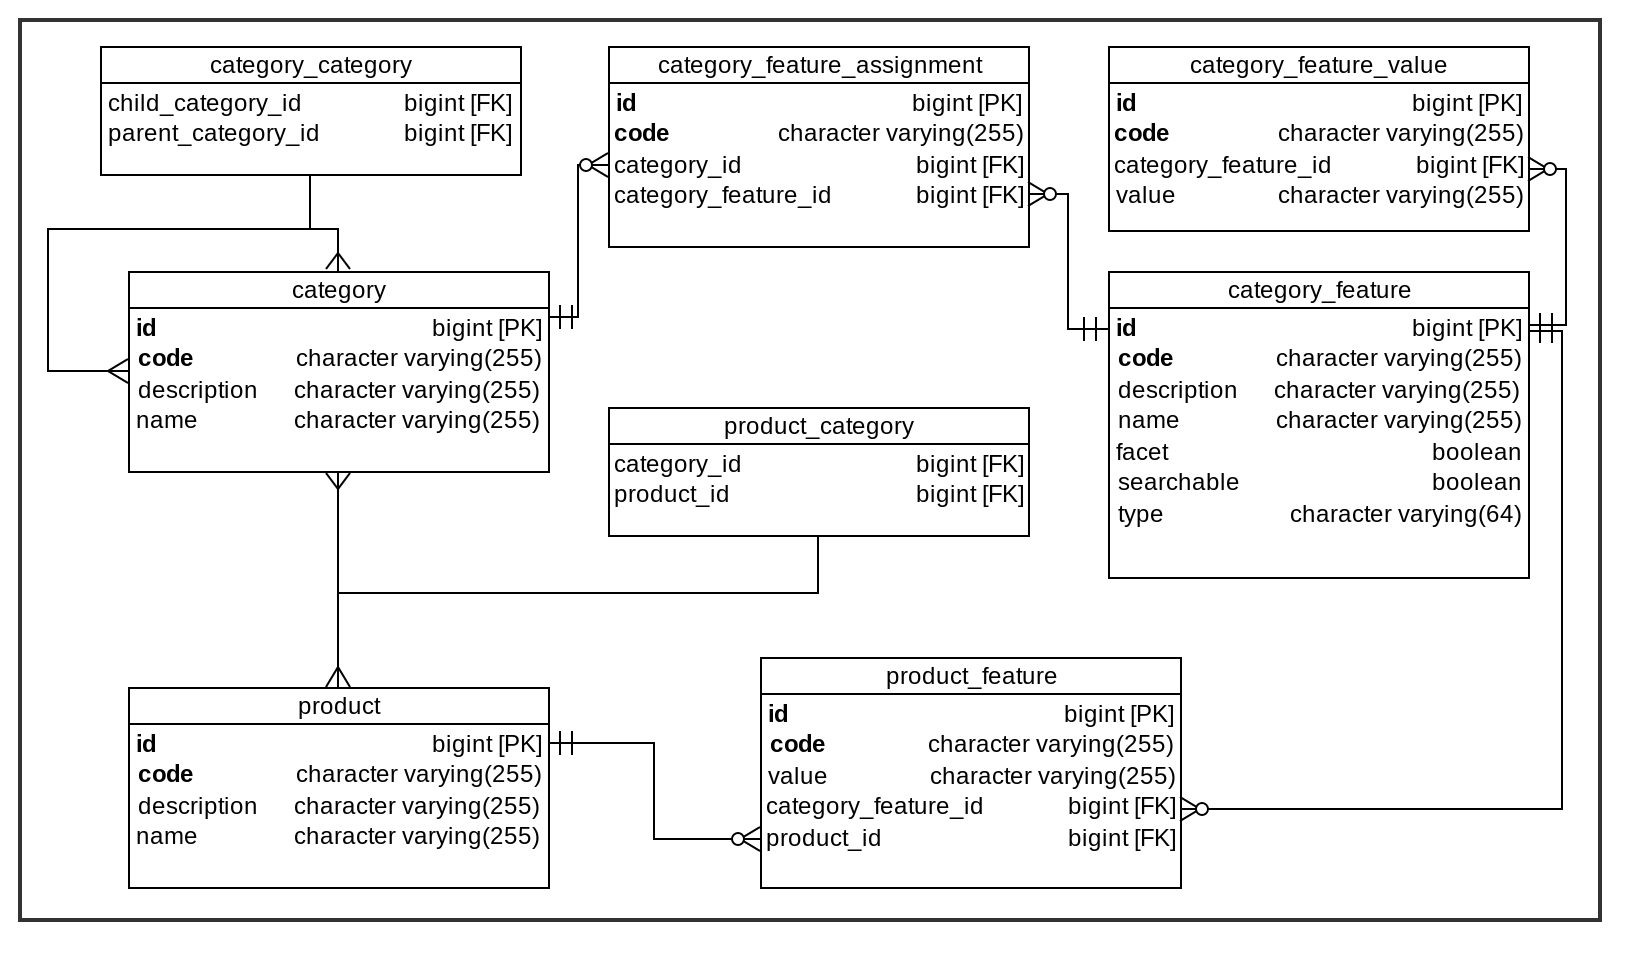
\includegraphics[scale=0.3]{db_sysKlas.png}
	\end{center}
	\caption{{\color{black}Diagram fragmentu bazy danych odpowiadającego za menu}} \label{db_sysKlas}
\end{figure}

\subsection{Mechanizm uprawnień}
Rysunek \ref{db_uprawnienia} przedstawia fragment bazy danych odpowiedzialny za obsługę uprawnień w panelu administracyjnym. Tabela \texttt{admin\_user} zawiera rekordy z użytkownikami administracyjnymi, którzy mogą zalogować się do systemu. Jest ona w relacji many to many z \texttt{admin\_permission}, co oznacza, że użytkownik administracyjny może mieć wiele uprawnień, jak i jedno uprawnienie może być przypisane do wielu użytkowników. Dodatkowo \texttt{admin\_permission} posiada kolumnę \texttt{class\_name} z nazwą klasy w systemie, której dotyczy uprawnienie. Aby stworzyć możliwość dziedziczenia uprawnień i układania ich w grupy, dodano klucz obcy \texttt{parent\_permission\_id} tworząc relację one to many do samego siebie. W ten sposób można tworzyć z uprawnień drzewiaste struktury -- oczywiście przy założeniu niewystępowania cykli. 

\begin{figure}
	\begin{center}
		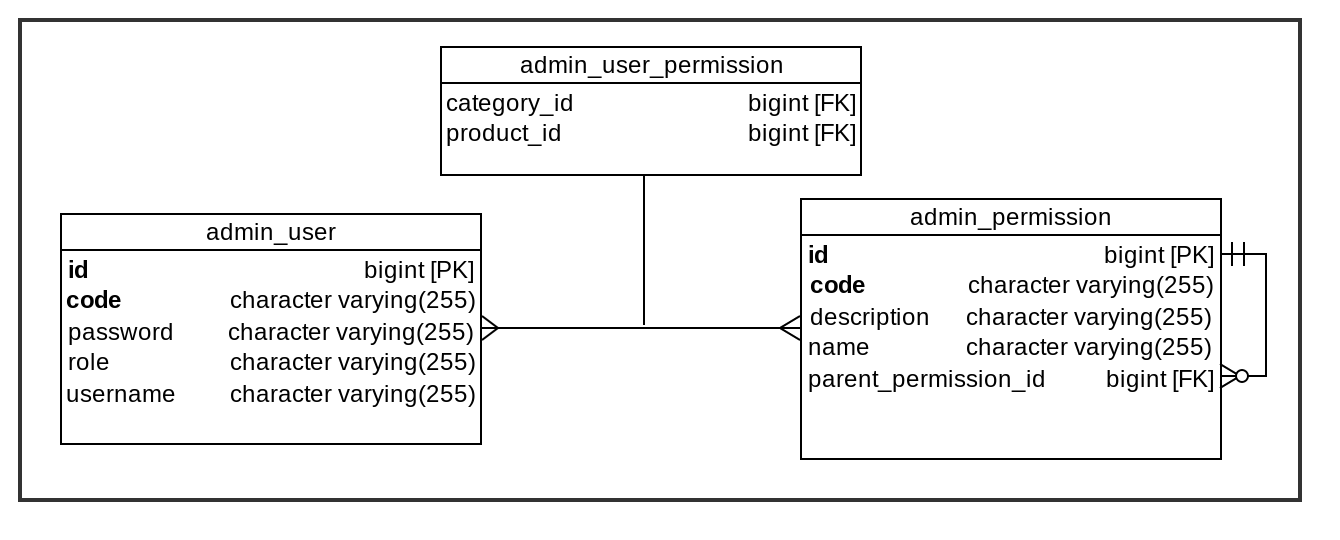
\includegraphics[scale=0.3]{db_uprawnienia.png}
	\end{center}
	\caption{{\color{black}Diagram fragmentu bazy danych odpowiadającego za uprawnienia w panelu administracyjnym}} \label{db_uprawnienia}
\end{figure}

\subsection{Proces zakupowy}
Diagram na rysunku \ref{db_zakup} przedstawia tabele bazodanowe, które biorą udział w procesie składania zamówienia. Oczywistymi elementami są tabele \texttt{customer i address}, powiązane relacją many to many. Zawierają one niezbędne szczegóły, które potrzebne są przy składaniu zamówień. Tabela \texttt{order} natomiast odpowiada systemowemu koszykowi, posiada klucz obcy \texttt{customer\_id}, co oznacza, że jest w relacji one to many z klientem. Daje to klientowi możliwość składania wielu zamówień. Jest ona również w relacji one to many (tym razem jako rodzic) z tabelą \texttt{order\_item}.  Ta reprezentuje jeden produkt dodany do koszyka w dowolnej ilości (za sprawą kolumny \texttt{quantity}). \texttt{order\_item} posiada również relację one to one do tabeli \texttt{archival\_product}, które pełni w sysetmie rolę archiwum produktowego, tak aby przy hipotetycznym usunięciu produktu ze sklepu zamówienie, które zostało już złożone nie zmieniło się. W celu utrzymania największej elastyczności w opisie archiwalnego produktu, stworzono dla niego w relacji one to many tabelę \texttt{archival\_product\_attributes}, do której jest możliwość zapisania prawie wszsytkich cech oryginalnego produktu. Te dwie tabele to przykład na to, jak może zostać zapisana w bazie danych mapa klucz-wartość.  

\begin{figure}
	\begin{center}
		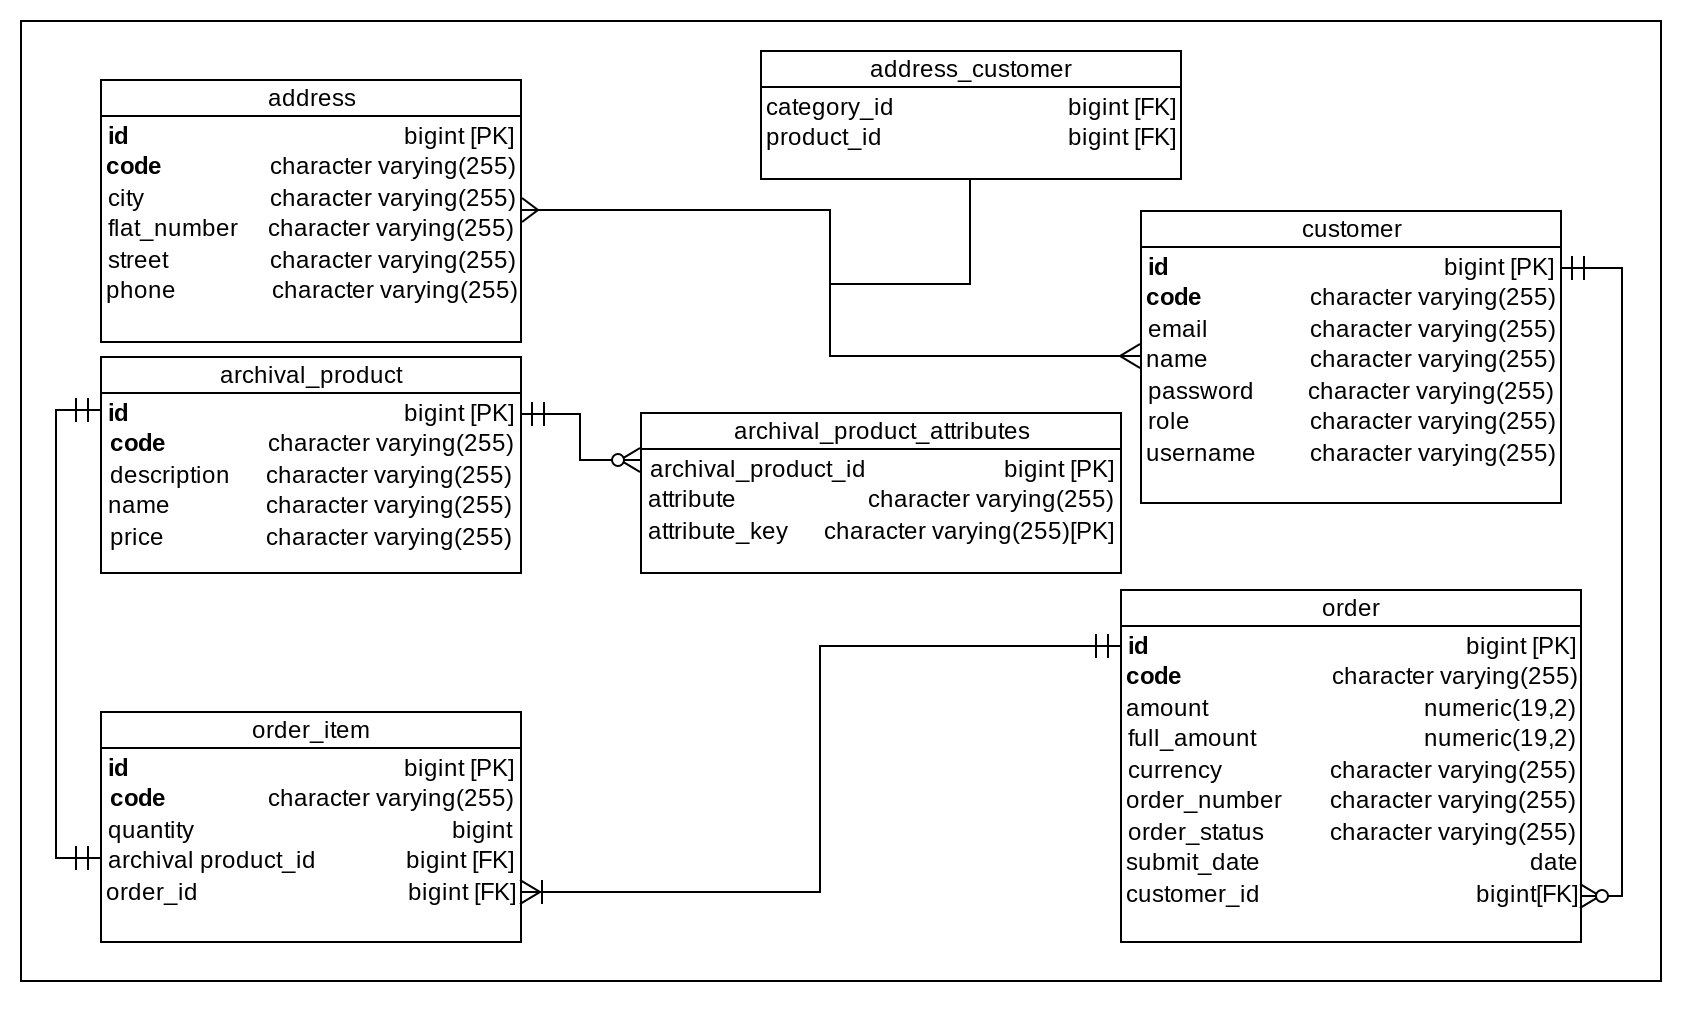
\includegraphics[scale=0.28]{db_zakup.png}
	\end{center}
	\caption{{\color{black}Diagram fragmentu bazy danych odpowiadającego za uprawnienia w panelu administracyjnym}} \label{db_zakup}
\end{figure}

\subsection{Połączenie bazy relacyjnej z płaską strukturą noSQL Apache Solr}
W tym podrozdziale został opisany mechanizm wyszukiwania od strony bazodanowej. Na diagramie \ref{db_wyszukiwarka} znajduje się diagram fragmentu relacyjnej bazy danych, w których znajdują się atrybuty produktowe, biorące udział w procesie wyszukiwania. Tabele na tym diagramie zostały opisane już w poprzednich podrozdziałach, jednak celem tego diagramu jest pokazanie, z jak wielu tabel pochodzą atrybuty produktowe i jak skomplikowane są połączenia między nimi. Niemożliwe jest aby system był w stanie za każdym wyszukaniem przez klienta wyciągać z relacyjnej bazy taką ilość danych. Byłoby to bardzo obciążające dla serwera. Dlatego podczas opisanego w poprzednich rozdziałach procesu indeksacji, który odbywa się w systemie raz na 15 minut, dane te są zbierane i produkty wraz ze wszystkimi ich atrybutami są wysyłane do nierelacyjnej bazy danych Apache Solr. Każdy produkt odpowiada jednemu dokumentowi w strukturze Solra. Takie rozwiązanie jest istotnie szybsze dlatego, że:
\begin{itemize}
	\item unikamy klasycznych połączeń bazodanowych, które są zwykle transakcyjne, co jest kosztowne czasowo
	\item unikamy kwerend z JOIN'ami, które często sprowadzają się do iloczynu kartezjańskiego, który również jest bardzo kosztowny
	\item Solr korzysta z silnika Lucene, który indeksuje każde słowo w każdym dokumencie, dlatego kwerenda jednosłowna z jednym dokumentem daje złożoność O(1). W miarę wzrostu danych złożoność wyszukiwania jest liniowa, gdyż przy każdym wyszukaniu skanowany jest każdy dokument. W przypadku relacyjnej bazy danych przy wzroście ilości rekordów, drastycznie spada wydajność ze względu na konieczność użycia JOIN'ów.
\end{itemize}
 
\begin{figure}
	\begin{center}
		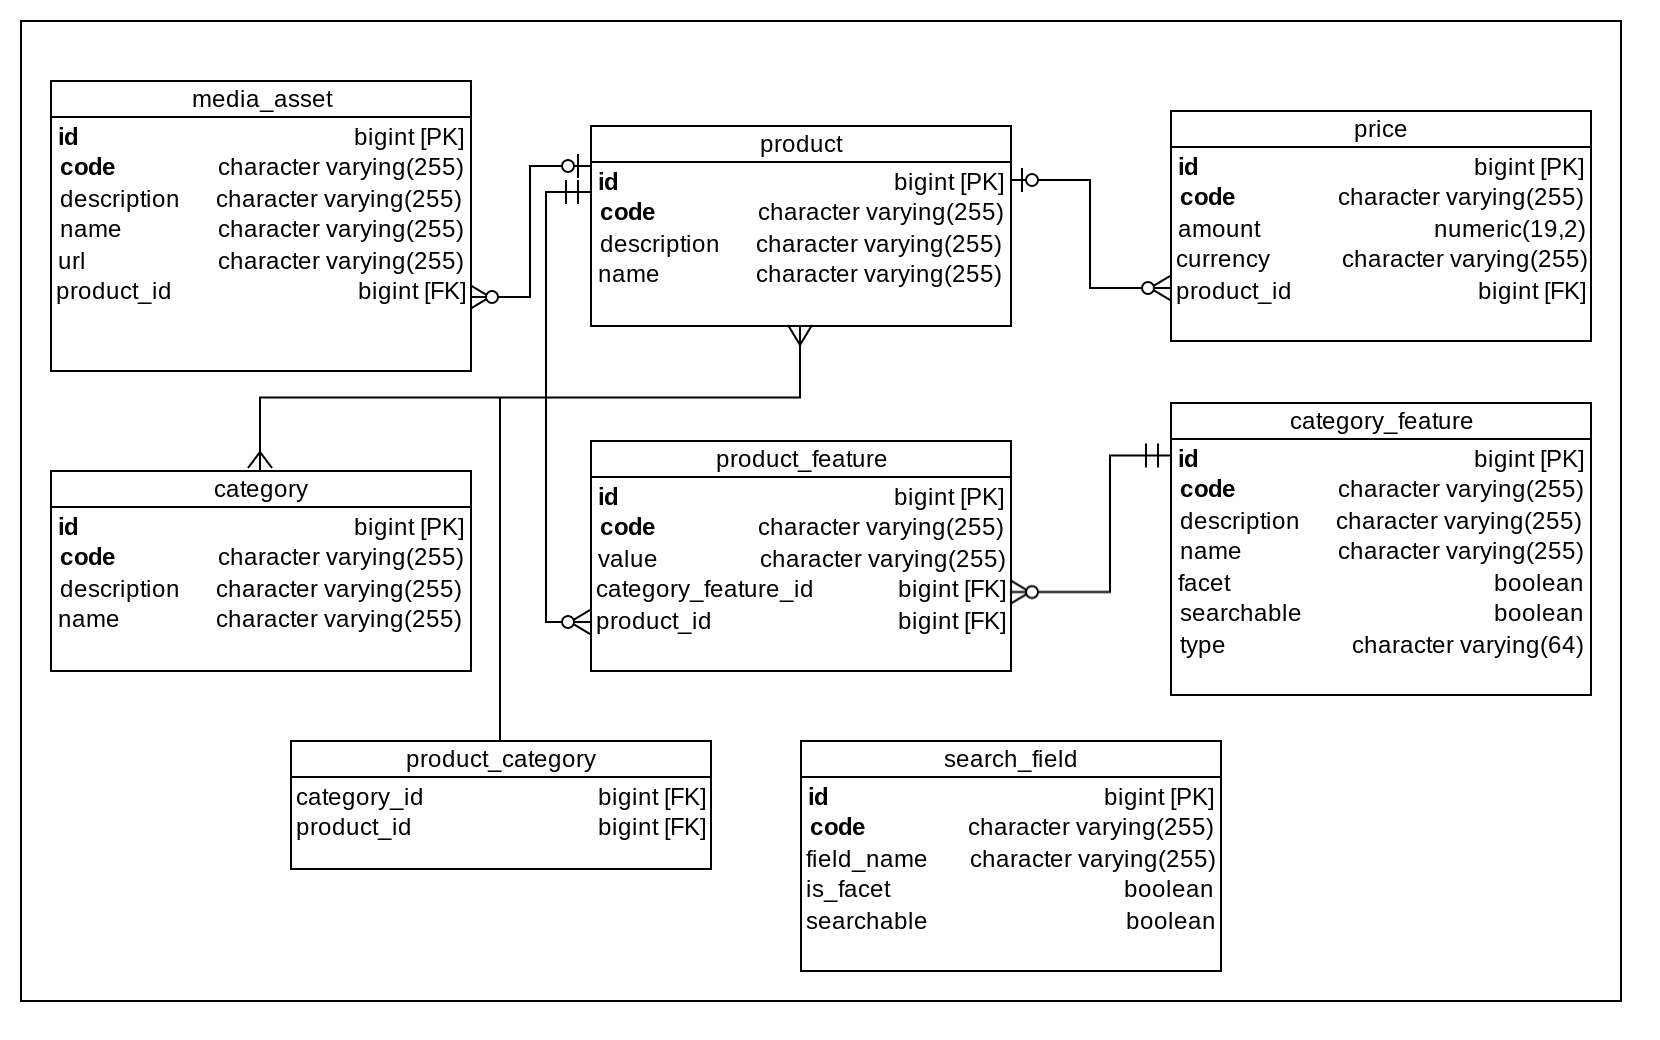
\includegraphics[scale=0.25]{db_wyszukiwarka.png}
	\end{center}
	\caption{{\color{black}Diagram fragmentu bazy danych skąd zbierane są atrybuty produktowe}} \label{db_wyszukiwarka}
\end{figure}


\subsection{System utrzymania bazy danych}
Jako system utrzymania bazy danych został wybrany PostgreSQL. Głównym powodem jest to, że uchodzi on za lepiej spisujący się do dużych baz danych (które mogą pojawić się w platfromie e-commerce). Bywa używany w projektach zawierających hurtownie danych, i które są nastawione na bardzo szybki zapis i odczyt.  Dodatkowo Hibernate\footnote{Hibernate -- framework w Javie do komunnikacji z bazą danych} jest łatwo konfigurowalny dla baz opartych o PostgreSQL. Ważną zaletą tego systemu jest także spełnienie właściwości transakcji według ACID (Atomicity, Consistency, Isolation, Durability). Spełnienie tych właściwości gwarantuje brak zagubionych lub błędnych danych w razie awarii systemu. 

\subsection{Normalizacja bazy danych}
Tabele zawarte w systemie są w trzeciej postaci normalnej. Wynika to z tego, że do tworzenia schematu bazy danych zostało wykorzystane mapowanie relacyjno-obiektowe, które same w sobie nie zapewnia 3NF, jednak sposób implementowania encji w standardzie JPA narzuca ją domyślnie. Każda tabela ma swój klucz główny oraz jest odzwierciedleniem pól w danej klasie - spełnienie 1NF, każda kolumna powinna być atomowa, przechowywać tylko jedną informację. Dodatkowo jedna encja w systemie oznacza jedną tabelę w bazie danych, co jest zgodne z 2NF, czyli wszystkie niekluczowe kolumny w tabeli muszą dotyczyć konkretnej klasy. 3NF jest również spełniona, ponieważ w żadnej z tabel nie ma niekluczowych informacji, które zależałyby od innych niekluczowych informacji. Wprowadzająca zamieszanie może być w tym przypadku tabela \texttt{order} z kolumną \texttt{full\_amount}, która zależy od ilości i ceny produktów, jednak te informacje znajdują się w innych tabelach, przez co 3NF jest zachowana. 
